% ============================================================================
% MAIN.TEX: SCIE3314 APSIM Tutorial
% ============================================================================
% Root document that compiles all modules, exercises, and appendices
% 
% COMPILATION:
%   pdflatex main.tex
%   bibtex main
%   pdflatex main.tex
%   pdflatex main.tex
%
% Or use latexmk: latexmk -pdf main.tex

% ============================================================================
% PREAMBLE: SCIE3314 APSIM Tutorial
% ============================================================================
% Packages, formatting, custom commands, and styling

\documentclass[12pt, a4paper, oneside]{book}

% ============================================================================
% CORE PACKAGES
% ============================================================================
\usepackage[utf8]{inputenc}
\usepackage[T1]{fontenc}
\usepackage[margin=2.5cm, top=2.5cm, bottom=2.5cm]{geometry}
\usepackage{fancyhdr}
\usepackage{setspace}
\onehalfspacing  % 1.5 line spacing for readability

% ============================================================================
% TYPOGRAPHY & COLORS
% ============================================================================
\usepackage{xcolor}
\usepackage{listings}
\usepackage{courier}
\usepackage{lmodern}
\usepackage{microtype}
\usepackage{helvet}

% Color definitions
\definecolor{darkblue}{rgb}{0.0, 0.0, 0.5}
\definecolor{codegreen}{rgb}{0.0, 0.5, 0.0}
\definecolor{codered}{rgb}{0.8, 0.0, 0.0}
\definecolor{codegray}{rgb}{0.5, 0.5, 0.5}
\definecolor{lightgray}{rgb}{0.95, 0.95, 0.95}

% UWA Brand Colours
\definecolor{UWABlue}{RGB}{33, 64, 154}
\definecolor{UWAGold}{RGB}{221, 177, 10}
\definecolor{UWAGrey}{RGB}{77, 77, 79}
\definecolor{UWALightBlue}{RGB}{228, 234, 249}
\definecolor{UWALightGold}{RGB}{253, 247, 215}
\definecolor{APSIMGreen}{RGB}{0, 120, 60}
\definecolor{WarningRed}{RGB}{180, 30, 30}

% ============================================================================
% MATHEMATICS & SCIENCE
% ============================================================================
\usepackage{amsmath}
\usepackage{amssymb}
\usepackage{siunitx}

% ============================================================================
% FIGURES & TABLES
% ============================================================================
\usepackage{graphicx}
\usepackage{array}
\usepackage{tabularx}
\usepackage{booktabs}
\usepackage{float}
\usepackage{caption}
\usepackage{subcaption}
\usepackage{multirow}
\usepackage{parskip}
\usepackage{tikz}
\usetikzlibrary{shapes.geometric, arrows.meta, positioning, calc, fit, backgrounds}
\usepackage{forest}

% Figure placement
\captionsetup{labelfont=bf, textfont=normalfont}
\renewcommand{\figurename}{Figure}
\renewcommand{\tablename}{Table}

% ============================================================================
% HYPERLINKS & REFERENCES
% ============================================================================
\usepackage[colorlinks=true, linkcolor=darkblue, citecolor=darkblue, urlcolor=darkblue]{hyperref}
\usepackage[noabbrev]{cleveref}

% ============================================================================
% CODE LISTINGS (for APSIM JSON, JavaScript, etc.)
% ============================================================================
\lstset{
  basicstyle=\ttfamily\small,
  breaklines=true,
  showstringspaces=false,
  commentstyle=\color{codegray},
  keywordstyle=\color{darkblue},
  stringstyle=\color{codegreen},
  backgroundcolor=\color{lightgray},
  frame=single,
  numbers=left,
  numberstyle=\tiny\color{codegray},
  rulecolor=\color{codegray},
  captionpos=b
}

% ============================================================================
% CUSTOM COMMANDS & ENVIRONMENTS
% ============================================================================

% Box for key concepts
\usepackage{tcolorbox}
\newtcolorbox{keyconceptbox}{
  colback=blue!5!white,
  colframe=darkblue,
  boxsep=5pt,
  left=5pt,
  right=5pt,
  top=5pt,
  bottom=5pt,
  arc=2mm
}

% Box for warnings/important notes
\newtcolorbox{warningbox}{
  colback=red!5!white,
  colframe=red,
  boxsep=5pt,
  left=5pt,
  right=5pt,
  top=5pt,
  bottom=5pt,
  arc=2mm
}

% Box for tips
\newtcolorbox{tipbox}{
  colback=green!5!white,
  colframe=codegreen,
  boxsep=5pt,
  left=5pt,
  right=5pt,
  top=5pt,
  bottom=5pt,
  arc=2mm
}

% Command for APSIM terms (monospace, styled)
\newcommand{\apsimterm}[1]{\texttt{\color{darkblue}#1}}

% Command for file names
\newcommand{\filename}[1]{\texttt{#1}}

% Command for variable names
\newcommand{\variable}[1]{\texttt{\color{codegreen}#1}}

% Command for parameter descriptions
\newcommand{\param}[2]{\textbf{#1:} \textit{#2}}

% ============================================================================
% HEADERS & FOOTERS
% ============================================================================
\pagestyle{fancy}
\fancyhf{}
\fancyhead[L]{\textit{SCIE3314 APSIM Tutorial}}
\fancyhead[R]{\textit{\nouppercase{\leftmark}}}
\fancyfoot[C]{\thepage}
\renewcommand{\headrulewidth}{0.4pt}
\renewcommand{\footrulewidth}{0.4pt}

% ============================================================================
% CHAPTER & SECTION FORMATTING
% ============================================================================
\usepackage{titlesec}
\titleformat{\chapter}[display]
  {\normalfont\LARGE\bfseries\color{darkblue}}
  {\chaptertitlename\ \thechapter}{20pt}{\LARGE}

\titleformat{\section}
  {\normalfont\Large\bfseries\color{darkblue}}
  {\thesection}{1em}{}

\titleformat{\subsection}
  {\normalfont\large\bfseries}
  {\thesubsection}{1em}{}

\titlespacing*{\chapter}{0pt}{-50pt}{30pt}
\titlespacing*{\section}{0pt}{12pt}{6pt}
\titlespacing*{\subsection}{0pt}{10pt}{4pt}

% ============================================================================
% TABLE OF CONTENTS FORMATTING
% ============================================================================
\usepackage{tocloft}
\setcounter{tocdepth}{2}

% ============================================================================
% BIBLIOGRAPHY & REFERENCES
% ============================================================================
% Bibliography: use basic bibtex (thebibliography env in main.tex)
% \usepackage[style=authoryear, backend=bibtex]{biblatex}
% \addbibresource{references.bib}

% ============================================================================
% MISCELLANEOUS
% ============================================================================
\usepackage{enumitem}
\setlist[itemize]{topsep=4pt, itemsep=2pt}
\setlist[enumerate]{topsep=4pt, itemsep=2pt}

% Reduce spacing around equations
\setlength{\abovedisplayskip}{6pt}
\setlength{\belowdisplayskip}{6pt}

% ============================================================================
% END PREAMBLE
% ============================================================================


\title{%
  \textbf{SCIE3314: Agricultural Production Systems Simulator (APSIM)} \\
  \large Introductory Tutorial \\
  \normalsize Modular Design for Crop Modelling and Decision Support
}

\author{
  School of Agriculture and Food Science \\
  University of Queensland \\
  \texttt{s.instructor@uq.edu.au}
}

\date{May 2026 \\ Version 1.0}

\begin{document}

% ============================================================================
% FRONT MATTER
% ============================================================================

\frontmatter

% Title page
\maketitle

% ============================================================================
% ACKNOWLEDGMENTS
% ============================================================================

\chapter*{Acknowledgments}

This tutorial was developed with reference to:
\begin{itemize}
  \item APSIM Next Gen 2025.6.7774.0 documentation
  \item APSOIL soil database (Australian soils)
  \item Weather files from BOM/SILO networks
  \item Pedagogic design based on Bloom's taxonomy and constructivist learning principles
\end{itemize}

We acknowledge the APSIM Initiative (CSIRO, QAAFI, CIMMYT, ICRISAT, Michigan State University) for developing and maintaining APSIM as a public good.

% ============================================================================
% TABLE OF CONTENTS, FIGURES, TABLES
% ============================================================================

\tableofcontents
\listoffigures
\listoftables

% ============================================================================
% PREFACE
% ============================================================================

\chapter*{Preface}

This tutorial introduces APSIM (Agricultural Production Systems Simulator), a process-based crop modelling platform widely used in research, extension, and operational decision support.

\begin{keyconceptbox}
\textbf{Learning Outcomes:}
After completing this tutorial, students will be able to:
\begin{enumerate}
  \item Understand the structure and daily sequence of APSIM simulations
  \item Configure and run crop simulations for decision analysis
  \item Interpret model outputs and assess crop responses to management
  \item Apply APSIM to explore agronomic questions (N fertilisation, phenology, variability)
  \item Troubleshoot common errors and validate simulation logic
\end{enumerate}
\end{keyconceptbox}

\section*{How to Use This Tutorial}

\textbf{For Instructors:} Each module (0--7) is designed as a 30--90 minute class session or self-study unit. Four integrated exercises (A--D) scaffold hands-on simulation work, progressing from simple water balance to multi-year variability analysis. All exercises use near-solved .apsimx files (components pre-configured; students modify parameters).

\textbf{For Students:} Start with Module 0 (Why APSIM?), then progress sequentially through Modules 1--7. Complete Exercises A--D in parallel or after each module block. Each module includes key concepts, worked examples, and links to reference entities in the LLM Wiki (\textit{see \cref{sec:wiki-resources}}).

\textbf{Prerequisites:} Basic agronomy (crop growth stages, soil water, nitrogen cycling). No programming required; JavaScript Manager rules are provided as templates.

% ============================================================================
% MAIN MATTER
% ============================================================================

\mainmatter

% ============================================================================
% MODULE 0: WHY APSIM?
% ============================================================================

% ============================================================================
% MODULE 0: WHY APSIM?
% ============================================================================
% Duration: 30 minutes (standalone or intro)
% Learning Goals: Motivation; overview; career relevance
% Prerequisites: None

\chapter{Module 0: Why APSIM?}
\label{ch:module0}

\section{Learning Objectives}

By the end of this module, you will:
\begin{itemize}
  \item Understand what crop modelling is and why it matters
  \item Identify key applications of APSIM in research, extension, and industry
  \item See APSIM in context alongside other simulation tools
  \item Recognize how APSIM connects to agronomic decision-making
\end{itemize}

\section{What is Crop Modelling?}

\begin{keyconceptbox}
\textbf{Crop Modelling} is the use of mathematical equations and computational models to simulate crop growth, development, and yield in response to weather, soil, and management decisions.
\end{keyconceptbox}

\subsection{Why Not Just Experiment?}

Field experiments are essential but have limitations:
\begin{itemize}
  \item \textbf{Time:} Experiments take seasons or years; models run in seconds
  \item \textbf{Cost:} Field trials are expensive; simulations are cheap
  \item \textbf{Scope:} Can't test every scenario; models explore hypotheticals
  \item \textbf{Climate:} Can't control weather; models test under different climates
  \item \textbf{Generalization:} Results from one site may not apply elsewhere; models extrapolate
\end{itemize}

Example: To test 5 sowing dates × 6 N rates × 3 varieties across 10 locations and 20 years of weather = 18,000 simulated scenarios. Field trials would take decades and millions of dollars.

\subsection{What Can Models Do?}

\begin{tipbox}
Crop models allow farmers, agronomists, and researchers to:
\begin{itemize}
  \item \textbf{Predict yield} under different management and climate scenarios
  \item \textbf{Optimize decisions} (N rate, sowing date, variety choice)
  \item \textbf{Assess risk} (variability across seasons; climate change impacts)
  \item \textbf{Understand mechanisms} (why does N affect grain protein?)
  \item \textbf{Train decisions support systems} (operational use in farms/regions)
\end{itemize}
\end{tipbox}

\section{APSIM: Overview}

APSIM (Agricultural Production Systems Simulator) is a process-based crop modelling platform developed by:
\begin{itemize}
  \item CSIRO (Australia)
  \item QAAFI (University of Queensland)
  \item CIMMYT (Mexico)
  \item ICRISAT (India)
  \item Michigan State University (USA)
\end{itemize}

\subsection{Key Features}

\begin{description}
  \item[\textbf{Process-based}] Models mechanistic interactions (photosynthesis, phenology, nutrient cycling), not just empirical curves
  \item[\textbf{Multi-component}] Soil water, nitrogen, phosphorus, organic matter, crops, weather, management all coupled
  \item[\textbf{Daily timestep}] High resolution for capturing short-term processes (daily rain, daily stress)
  \item[\textbf{Modular}] Can mix-and-match components; run in research mode or farmer decision-support mode
  \item[\textbf{Open-source}] Free; community-maintained; thousands of users worldwide
  \item[\textbf{Validated}] Decades of testing against field data across 100+ crop types and locations
\end{description}

\section{APSIM in Action: Real-World Applications}

\subsection{Research Example: Climate Change Impact on Wheat Yield}

A researcher wants to know: \textit{How will wheat yields change if rainfall decreases by 20\% and temperatures increase by 2°C?}

\begin{enumerate}
  \item Set up APSIM with current weather and soils for a wheat-growing region
  \item Run baseline simulation (100 years of current climate)
  \item Run scenario simulation (same 100 years but weather modified)
  \item Compare yield distributions: baseline vs. scenario
  \item Identify adaptation strategies (earlier sowing? different variety? more irrigation?)
\end{enumerate}

\subsection{Extension Example: Nitrogen Rate Optimization}

An extension officer works with 50 wheat farmers in a district. Question: \textit{What N rate maximizes profit for different soil types and seasons?}

\begin{enumerate}
  \item Map farmer soils; input into APSIM
  \item Run 5 N rates (0, 50, 100, 150, 200 kg/ha) × 20 years of regional weather
  \item Calculate yield response and NUE (Nitrogen Use Efficiency)
  \item Assess profit = Yield $\times$ Grain Price $-$ N Cost
  \item Recommend N rate based on soil, season outlook, grain price
\end{enumerate}

\subsection{Operational Example: Sowing Decision Support}

A farmer has a sowing window (May 1–July 10) and wants to know: \textit{When should I sow to maximize yield?}

\begin{enumerate}
  \item Set up APSIM with farm soil, local weather data (or forecast)
  \item Sow on different dates; track emergence, phenology, water availability, final yield
  \item Provide decision rule: ``Sow when ESW > 100 mm AND recent rain > 25 mm''
  \item Embed this rule in farm decision-support app; farmer checks conditions daily
\end{enumerate}

\section{APSIM Compared to Other Tools}

\begin{table}[H]
\centering
\caption{Comparison of Crop Modelling Platforms}
\label{tab:model-comparison}
\begin{tabularx}{\textwidth}{l|X|X|X|X}
\toprule
\textbf{Feature} & \textbf{APSIM} & \textbf{DSSAT} & \textbf{RZWQM} & \textbf{AquaCrop} \\
\midrule
Process-based & Yes & Yes & Yes & Simplified \\
Multi-crop & 100+ & 40+ & 10+ & 30+ \\
N cycling & Yes & Yes & Yes & Limited \\
Climate datasets & Global & Global & Limited & Global \\
User interface & GUI + scripting & DOS/Web & Command-line & GUI \\
Cost & Free & Free & Free & Free \\
Learning curve & Steep & Moderate & Steep & Gentle \\
Active community & Large & Moderate & Small & Moderate \\
\bottomrule
\end{tabularx}
\end{table}

\begin{warningbox}
\textbf{Note:} APSIM has a steeper learning curve but offers more flexibility and detail. AquaCrop is simpler but less mechanistic. DSSAT is similar to APSIM but different design philosophy. Choose based on your research question and available data.
\end{warningbox}

\section{Key Concepts in APSIM}

\subsection{Daily Simulation Loop}

APSIM runs a daily timestep cycle:

\begin{enumerate}
  \item \textbf{Clock advances} by one day
  \item \textbf{Weather data} is read (temperature, rainfall, radiation)
  \item \textbf{Manager evaluates rules} (is it time to sow? fertilise? harvest?)
  \item \textbf{Soil processes} calculate water, N availability
  \item \textbf{Crop model} calculates growth, N uptake, phenology
  \item \textbf{Report} outputs selected variables
  \item Repeat
\end{enumerate}

\subsection{Three-Layer Problem Representation}

APSIM separates concerns:

\begin{description}
  \item[\textbf{State layer}] What is the current soil water, N pool, crop biomass, stage?
  \item[\textbf{Process layer}] How do these states change? (PET, infiltration, phenology equations)
  \item[\textbf{Driver layer}] What drives change? (Weather, management decisions)
\end{description}

This allows researchers to:
\begin{itemize}
  \item Test process implementations in isolation
  \item Swap components (use different crop model, different soil model)
  \item Understand cause-effect pathways
\end{itemize}

\section{Career Relevance}

Crop modelling skills are in demand:

\begin{itemize}
  \item \textbf{Research}: Universities, CSIRO, international agricultural research centers
  \item \textbf{Extension}: Government agencies, agricultural services, extension providers
  \item \textbf{Private sector}: Agribusiness, fertiliser companies, crop input providers
  \item \textbf{Policy}: Climate adaptation; food security; natural resource management
  \item \textbf{Operations}: Farm management software companies; decision support platforms
\end{itemize}

\begin{keyconceptbox}
\textbf{Key Takeaway:} APSIM is a professional tool used globally in research, extension, and operations. Learning APSIM opens careers in agricultural science and decision support.
\end{keyconceptbox}

\section{Roadmap for This Tutorial}

This tutorial is structured in 8 modules:

\begin{description}
  \item[\textbf{Module 0}] Why APSIM? (this module) — motivation and overview
  \item[\textbf{Module 1}] Structure — APSIM's component architecture
  \item[\textbf{Module 2}] First Simulation — run a simple fallow water balance
  \item[\textbf{Module 3}] Output Analysis — interpret simulation results
  \item[\textbf{Module 4}] Nitrogen Fertilisation — explore N response curves
  \item[\textbf{Module 5}] Phenology \& Thermal Time — understand crop development
  \item[\textbf{Module 6}] Long-Term Variability — assess climate risk
  \item[\textbf{Module 7}] Climate Scenarios — explore adaptation strategies
\end{description}

Plus four hands-on exercises:
\begin{itemize}
  \item \textbf{Exercise A}: Fallow water balance (7 years)
  \item \textbf{Exercise B}: N response factorial (4 rates)
  \item \textbf{Exercise C}: Sowing date factorial (3 scenarios)
  \item \textbf{Exercise D}: 20-year variability analysis
\end{itemize}

\section{How APSIM Works: The Information Flow}

\begin{keyconceptbox}
\textbf{Process-Based Modelling:} A process-based model simulates the underlying biological and physical mechanisms (e.g., soil water flow, photosynthesis, nitrogen mineralisation). This contrasts with empirical models that fit statistical equations to observed data. Because APSIM represents mechanisms, it can be applied to conditions not included in its original calibration --- making it suitable for evaluating novel management strategies or future climate scenarios.
\end{keyconceptbox}

Figure~\ref{fig:apsim_concept} summarises how information flows through an APSIM simulation each day.

\begin{figure}[H]
\centering
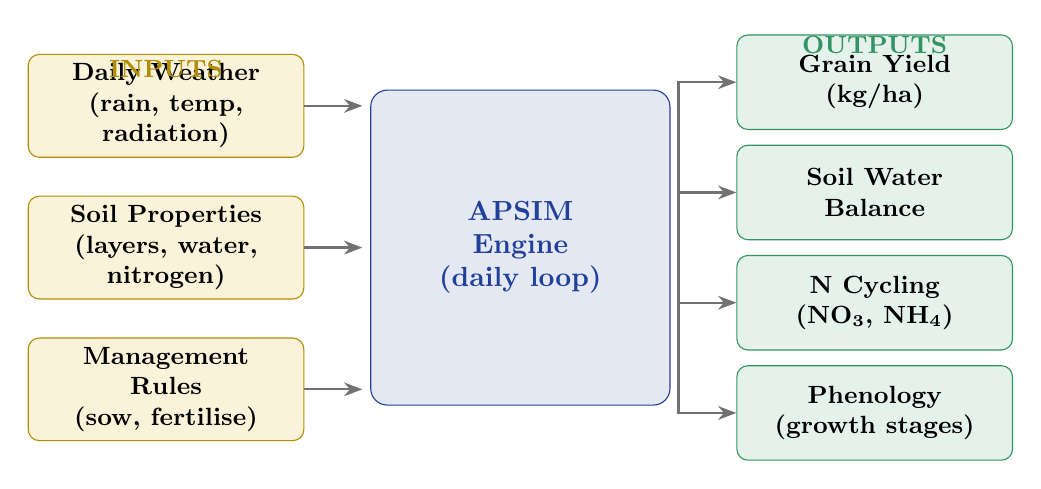
\begin{tikzpicture}[
  node distance=1.2cm and 2.2cm,
  inbox/.style={rectangle, rounded corners=4pt, draw=UWAGold!80!black,
    fill=UWAGold!15, minimum width=3.5cm, minimum height=1.2cm,
    align=center, font=\small\bfseries},
  corebox/.style={rectangle, rounded corners=6pt, draw=UWABlue,
    fill=UWABlue!12, minimum width=3.8cm, minimum height=4.0cm,
    align=center, font=\bfseries\color{UWABlue}},
  outbox/.style={rectangle, rounded corners=4pt, draw=APSIMGreen!80,
    fill=APSIMGreen!10, minimum width=3.5cm, minimum height=1.2cm,
    align=center, font=\small\bfseries},
  arr/.style={-Stealth, thick, color=UWAGrey!80}
]
  \node[inbox] (weather)  at (0, 1.8)  {Daily Weather\\(rain, temp,\\radiation)};
  \node[inbox] (soil)     at (0, 0)    {Soil Properties\\(layers, water,\\nitrogen)};
  \node[inbox] (mgmt)     at (0,-1.8)  {Management\\Rules\\(sow, fertilise)};

  \node[corebox] (core)   at (4.5, 0)  {APSIM\\Engine\\(daily loop)};

  \node[outbox] (yield)   at (9.0, 2.1) {Grain Yield\\(kg/ha)};
  \node[outbox] (water)   at (9.0, 0.7) {Soil Water\\Balance};
  \node[outbox] (n)       at (9.0,-0.7) {N Cycling\\(NO\textsubscript{3}, NH\textsubscript{4})};
  \node[outbox] (pheno)   at (9.0,-2.1) {Phenology\\(growth stages)};

  \draw[arr] (weather.east) -- ([xshift=-0.1cm]core.west |- weather);
  \draw[arr] (soil.east)    -- ([xshift=-0.1cm]core.west);
  \draw[arr] (mgmt.east)    -- ([xshift=-0.1cm]core.west |- mgmt);

  \draw[arr] ([xshift=0.1cm]core.east) |- (yield.west);
  \draw[arr] ([xshift=0.1cm]core.east) |- (water.west);
  \draw[arr] ([xshift=0.1cm]core.east) |- (n.west);
  \draw[arr] ([xshift=0.1cm]core.east) |- (pheno.west);

  \node[font=\small\bfseries\color{UWAGold!80!black}, anchor=north] at (0, 2.5) {INPUTS};
  \node[font=\small\bfseries\color{APSIMGreen!80},    anchor=north] at (9.0, 2.8) {OUTPUTS};
\end{tikzpicture}
\caption{Conceptual overview of an APSIM simulation. Daily inputs drive a process-based calculation engine, generating outputs on crop yield, soil water, nitrogen cycling, and crop phenology.}
\label{fig:apsim_concept}
\end{figure}

\section{Summary}

\begin{itemize}
  \item Crop models simulate crop-soil-weather-management interactions
  \item APSIM is a powerful, process-based platform with global adoption
  \item Applications span research, extension, and operational decision support
  \item This tutorial teaches APSIM through progressive modules + hands-on exercises
  \item Career pathways exist in research, extension, agribusiness, and policy
\end{itemize}

\section{What's Next?}

In Module 1, we dive into APSIM's structure: components, daily sequence, .apsimx file format, and how to interpret a simulation setup.

% ============================================================================
% END MODULE 0
% ============================================================================


% ============================================================================
% MODULE 1: STRUCTURE
% ============================================================================

% ============================================================================
% MODULE 1: STRUCTURE
% ============================================================================
% Duration: 60–90 minutes (foundational; reference the wheat_example.apsimx)
% Learning Goals: Understand APSIM architecture; .apsimx JSON format; daily sequence
% Prerequisites: Module 0

\chapter{Module 1: APSIM Structure}
\label{ch:module1}

\section{Learning Objectives}

By the end of this module, you will:
\begin{itemize}
  \item Understand APSIM's component hierarchy (Simulations $\to$ Simulation $\to$ Zone $\to$ Components)
  \item Recognize the daily execution sequence (Clock $\to$ Weather $\to$ Manager $\to$ Soil $\to$ Crop $\to$ Report)
  \item Interpret a \filename{.apsimx} JSON file structure
  \item Understand the role of each component (Clock, Weather, Soil, Wheat, Manager, Report, DataStore)
  \item Navigate APSIM's GUI to view and modify simulation structure
\end{itemize}

\section{APSIM's Component Architecture}

\subsection{Hierarchy}

APSIM organizes all simulation information in a nested hierarchy:

\begin{center}
\begin{verbatim}
Simulations (root)
  └─ Simulation 1
      ├─ Global Components
      │   ├─ Clock
      │   ├─ Weather
      │   ├─ SoilArbitrator
      │   └─ MicroClimate
      └─ Zone (Field)
          ├─ Report
          ├─ Fertiliser
          └─ Soil (with layers)
          ├─ Wheat (crop model)
          ├─ Manager (rule 1: sow)
          ├─ Manager (rule 2: fertilise)
          └─ Manager (rule 3: harvest)
\end{verbatim}
\end{center}

\begin{keyconceptbox}
\textbf{Key Principle:} Components are pluggable. You can swap components (different crop model, different soil model) without changing the overall structure.
\end{keyconceptbox}

\subsection{Global Components}

\begin{description}
  \item[\apsimterm{Clock}] Advances simulation by one day. Sets start date, end date, timestep (always 1 day in APSIM). Synchronizes all other components to daily updates.
  
  \item[\apsimterm{Weather}] Reads external weather file (\filename{.met} format). Provides daily maximum temperature, minimum temperature, rainfall, radiation, humidity, wind speed to all other components.
  
  \item[\apsimterm{SoilArbitrator}] Coordinates soil water and nutrient availability. When multiple processes access soil (e.g., plant root uptake, soil evaporation), arbitrator ensures consistency.
  
  \item[\apsimterm{MicroClimate}] Calculates energy balance at soil surface. Partitions radiation (direct vs. diffuse), interception, albedo, reference height effects.
\end{description}

\subsection{Zone Components}

A Zone represents a spatial patch (typically 1 hectare for field simulations). Multiple zones allow side-by-side comparisons (e.g., different management, different soil).

\begin{description}
  \item[\apsimterm{Soil}] Multi-layer soil profile. Contains physical properties (bulk density, water characteristics), organic matter, chemical properties (pH, nutrients), and initial conditions. Sub-components: Physical, SoilWater, Organic, Chemical, Nutrient (N cycle), solutes (NO\textsubscript{3}, NH\textsubscript{4}, Urea), Temperature.
  
  \item[\apsimterm{Wheat (or other Crop)}] Process-based crop model. Simulates phenology (thermal time, Zadok stages), biomass accumulation (photosynthesis, respiration), grain development, nutrient uptake, and stress responses.
  
  \item[\apsimterm{Manager}] User-defined management rules. Written in JavaScript or C\#; evaluated daily. Typical rules: sow when conditions met, apply fertiliser on date, harvest when physiologically mature.
  
  \item[\apsimterm{Fertiliser}] Component that applies nutrient inputs. Manager calls \variable{Fertiliser.Apply()} to add N, P, K at specified times.
  
  \item[\apsimterm{Report}] Output filter. Specifies which variables APSIM saves to the database. Reduces output file size by excluding irrelevant variables.
  
  \item[\apsimterm{DataStore}] Database (SQL-like) that receives daily reports and exports to Excel/CSV at simulation end.
\end{description}

\section{Daily Execution Sequence}

Each day, APSIM follows a strict sequence:

\begin{enumerate}
  \item \textbf{Clock.Today} advances by 1 day
  \item \textbf{Weather} reads data for today
  \item \textbf{Manager} evaluates and executes all rules
  \item \textbf{Soil} calculates water balance (infiltration, drainage, evaporation)
  \item \textbf{Wheat} calculates phenology, photosynthesis, N uptake, growth
  \item \textbf{Report} outputs selected variables to database
  \item \textbf{DataStore} receives report data
  \item Repeat (next day)
\end{enumerate}

\begin{warningbox}
\textbf{Important:} Order matters! Manager runs before Soil/Crop, so today's sowing decision uses yesterday's soil state. Soil runs before Crop, so water and N availability affect today's crop growth. This sequence is fundamental to APSIM.
\end{warningbox}

\section{The .apsimx File Format}

APSIM simulations are stored as JSON files (\filename{.apsimx}). Example structure:

\begin{lstlisting}[language=json, caption=Simplified .apsimx structure]
{
  "$type": "Models.Core.Simulations",
  "Name": "Simulations",
  "Children": [
    {
      "$type": "Models.Core.Simulation",
      "Name": "Simulation1",
      "Children": [
        {
          "$type": "Models.Clock",
          "Start": "1900-01-01",
          "End": "2000-12-31",
          "Name": "Clock"
        },
        {
          "$type": "Models.Climate.Weather",
          "FileName": "%root%/Examples/WeatherFiles/AU_Dalby.met",
          "Name": "Weather"
        },
        { ... more components ... }
      ]
    },
    {
      "$type": "Models.Storage.DataStore",
      "Name": "DataStore"
    }
  ]
}
\end{lstlisting}

\begin{keyconceptbox}
\textbf{Key Observation:} The JSON structure mirrors the component hierarchy. APSIM reads this file at startup, instantiates components, and establishes linkages. You can edit \filename{.apsimx} files directly in a text editor, but APSIM's GUI is more user-friendly.
\end{keyconceptbox}

\section{Component Reference Table}

\begin{table}[H]
\centering
\caption{APSIM Components: Role and Typical Configuration}
\label{tab:components}
\begin{tabularx}{\textwidth}{p{2cm}|p{3cm}|p{5cm}|p{2cm}}
\toprule
\textbf{Component} & \textbf{Type} & \textbf{Configuration} & \textbf{Ref} \\
\midrule
Clock & Input & Dates (start, end), timestep & \cref{sec:clock} \\
Weather & Input & File path (\filename{.met}), variables & \cref{sec:weather} \\
Soil & State & Layers, properties, initial water/N & \cref{sec:soil} \\
Wheat & Process & Phenology, LAI, grain fill & \cref{sec:wheat} \\
Manager & Control & Rules (JavaScript or C\#) & \cref{sec:manager} \\
Report & Output & Variable list & \cref{sec:report} \\
DataStore & Output & Database (auto-populated) & \cref{sec:datastore} \\
\bottomrule
\end{tabularx}
\end{table}

\section{Interpreting a Real Simulation: wheat\_example.apsimx}

We'll use \filename{wheat\_example.apsimx} (provided in \filename{Apsim\_examples/}) as a reference model.

\subsection{Key Configuration}

\begin{description}
  \item[\textbf{Location}] Dalby, Queensland (Black Vertosol soil)
  \item[\textbf{Climate}] 101 years (1900--2000) from SILO/BOM weather file
  \item[\textbf{Crop}] Wheat (Hartog cultivar), 120 plants/m\textsuperscript{2}
  \item[\textbf{Soil}] 7-layer profile, plant-available water = 361 mm
  \item[\textbf{Management}] 3 rules: sow (ESW > 100 mm + rain), fertilise (160 kg/ha N at sowing), harvest (at maturity)
\end{description}

\subsection{Output Variables}

Report tracks 13 daily variables:
\begin{itemize}
  \item Phenology: Zadok stage, stage name
  \item Growth: LAI, total biomass, grain mass
  \item Grain quality: Grain number, size, protein, N content
  \item Yield: Grain total weight
\end{itemize}

\section{Common Misconceptions}

\begin{warningbox}
\textbf{Misconception 1:} ``I can change timestep from daily to hourly.''

\textit{Reality:} APSIM is designed for daily timestep only. Many processes (phenology, root growth) are not parameterized for sub-daily resolution. If you need hourly resolution, consider alternative models (e.g., DSSAT in hourly mode, though rare).
\end{warningbox}

\begin{warningbox}
\textbf{Misconception 2:} ``Manager runs continuously, not daily.''

\textit{Reality:} Manager evaluates once per day (during the daily sequence). If you want multiple decisions per day (e.g., separate sowing and fertiliser decisions), both should be Manager rules that fire on the same day (order determined by rule sequence).
\end{warningbox}

\begin{warningbox}
\textbf{Misconception 3:} ``I can edit \filename{.apsimx} files without understanding JSON.''

\textit{Reality:} JSON is strict. Mismatched braces, quotes, or commas will cause APSIM to fail. Use APSIM's GUI to create files; edit manually only if you understand JSON syntax or use a JSON validator.
\end{warningbox}

\section{Navigating APSIM's GUI}

\subsection{Opening a Simulation}

\begin{enumerate}
  \item Launch APSIM
  \item File $\to$ Open $\to$ select \filename{.apsimx} file
  \item You should see a tree structure on the left (Components), properties panel on the right
\end{enumerate}

\subsection{Viewing Components}

\begin{itemize}
  \item Click on a component in the tree to view its properties
  \item Properties show all configurable parameters (dates, N rate, etc.)
  \item Some properties have dropdown menus (e.g., cultivar names, soil names)
\end{itemize}

\subsection{Running a Simulation}

\begin{enumerate}
  \item Select the Simulation in the tree
  \item Click the ``Run'' button (or Ctrl+R)
  \item APSIM displays progress in the output window
  \item When complete, click ``Generated Outputs'' or ``DataStore'' to view results
\end{enumerate}

\subsection{Exporting Results}

\begin{enumerate}
  \item Right-click the DataStore in the tree
  \item Select ``Export'' $\to$ ``To Excel'' or ``To CSV''
  \item Choose filename and location
  \item Results are now ready for analysis in Excel or Python
\end{enumerate}

\section{Summary}

\begin{itemize}
  \item APSIM structure: Hierarchy of components (Clock, Weather, Soil, Crop, Manager, Report, DataStore)
  \item Daily sequence: Clock $\to$ Weather $\to$ Manager $\to$ Soil $\to$ Crop $\to$ Report
  \item .apsimx file is JSON; mirrors component hierarchy
  \item Each component has specific role and configuration
  \item APSIM GUI provides user-friendly interface for viewing and modifying simulations
\end{itemize}

\section{Key Resources}

See the LLM Wiki for detailed reference pages:
\begin{itemize}
  \item [[Clock]] — Simulation timing
  \item [[Weather]] — Climate input
  \item [[Soil]] — Soil profile setup
  \item [[Wheat]] — Crop model
  \item [[Manager]] — Management rules
  \item [[Report]] — Output variables
  \item [[DataStore]] — Results database
\end{itemize}

\section{What's Next?}

In Module 2, you'll set up and run your first APSIM simulation: a simple fallow water balance.

% ============================================================================
% END MODULE 1
% ============================================================================


% ============================================================================
% MODULE 2: FIRST SIMULATION
% ============================================================================

% ============================================================================
% MODULE 2: FIRST SIMULATION
% ============================================================================
% Duration: 60 minutes (hands-on; near-solved file provided)
% Learning Goals: Set up, run, and interpret a fallow water balance simulation
% Prerequisites: Module 0, Module 1

\chapter{Module 2: First Simulation}
\label{ch:module2}

\section{Learning Objectives}

By the end of this module, you will:
\begin{itemize}
  \item Set up a simple APSIM simulation from scratch
  \item Understand fallow water balance: rainfall, runoff, drainage, evaporation
  \item Interpret daily ESW (extractable soil water) as an indicator of sowing readiness
  \item Run simulation and export results to Excel
  \item Troubleshoot common startup errors (file not found, missing dates, etc.)
\end{itemize}

\section{Conceptual Framework: Fallow Water Balance}

\subsection{What is a Fallow?}

A fallow is a season where the field is left without a crop. Soil water accumulates (useful before sowing) or is lost to drainage/evaporation.

\begin{keyconceptbox}
\textbf{Daily Water Balance Equation:}
\[
\text{ESW}_{t} = \text{ESW}_{t-1} + \text{Rainfall} - \text{Runoff} - \text{Drainage} - \text{Evaporation}
\]

where ESW = extractable soil water (mm), available for plant growth.
\end{keyconceptbox}

\subsection{When Are Soils Ready for Sowing?}

Farmers typically wait for:
\begin{itemize}
  \item ESW $>$ 100 mm (soil has adequate water to support germination and early growth)
  \item Rainfall $>$ 25 mm in last 7 days (recent rain indicates favorable conditions)
  \item Date within sowing window (e.g., May 1 – July 10 for winter wheat in Queensland)
\end{itemize}

Exercise A explores these thresholds using a 7-year fallow simulation.

\section{Getting Started: Open Exercise A}

\subsection{File Location}

\filename{Exercise\_A\_Fallow\_Water\_Balance.apsimx} (provided in course materials)

\subsection{Simulation Setup}

\textbf{Clock:} 7 years of a representative site (e.g., 1950–1957)

\textbf{Weather:} Dalby, Queensland (real BOM/SILO data)

\textbf{Soil:} Norwin Vertosol (black clay; realistic for wheat region)

\textbf{Management:} None (fallow = no crop, no fertiliser)

\textbf{Report Variables:} 
\begin{itemize}
  \item [Clock].Today (date)
  \item [Soil].ESW (extractable soil water)
  \item [Weather].Rainfall (daily rain)
  \item [Soil].SoilWater.Evaporation (simulated evaporation)
  \item [Soil].SoilWater.Drainage (deep percolation)
\end{itemize}

\section{Running the Simulation}

\subsection{Step 1: Open APSIM}

\begin{enumerate}
  \item Launch APSIM Next Gen
  \item File $\to$ Open $\to$ select \filename{Exercise\_A\_Fallow\_Water\_Balance.apsimx}
\end{enumerate}

\subsection{Step 2: View Structure}

\begin{itemize}
  \item Expand the tree on the left
  \item Verify components: Clock, Weather, Soil, Report, DataStore
  \item Click each component to check configuration (dates, file paths, variables)
\end{itemize}

\subsection{Step 3: Run Simulation}

\begin{enumerate}
  \item Click the Simulation in the tree
  \item Press Run button (or Ctrl+R)
  \item Watch the output window for progress
  \item Simulation should complete without errors
\end{enumerate}

\subsection{Step 4: View Results}

\begin{enumerate}
  \item Click DataStore in the tree
  \item Right-click $\to$ Export $\to$ To Excel
  \item Name file: \filename{Exercise\_A\_Results.xlsx}
  \item Open in Excel; examine data
\end{enumerate}

\section{Analyzing the Data}

\subsection{Key Columns}

\begin{table}[H]
\centering
\caption{Output Variables in Exercise A}
\label{tab:exercise-a-vars}
\begin{tabularx}{\textwidth}{l|X|X}
\toprule
\textbf{Column} & \textbf{Units} & \textbf{Interpretation} \\
\midrule
Clock.Today & Date & Calendar date \\
Soil.ESW & mm & Plant-available water; sowing threshold is ESW $>$ 100 mm \\
Weather.Rainfall & mm & Daily precipitation \\
Soil.SoilWater.Evaporation & mm & Soil water lost to atmosphere (PET if no crop) \\
Soil.SoilWater.Drainage & mm & Water percolating below root zone \\
\bottomrule
\end{tabularx}
\end{table}

\subsection{Analysis Prompts}

\begin{enumerate}
  \item \textbf{Seasonal Pattern:} Plot ESW vs. date across all 7 years. When does ESW peak? When is it lowest?
  
  \item \textbf{Sowing Window:} Identify dates when ESW $>$ 100 mm AND rainfall in last 7 days $>$ 25 mm. How many sowing opportunities per year?
  
  \item \textbf{Dry Year vs. Wet Year:} Compare ESW profiles for a dry year vs. wet year. What drives the difference?
  
  \item \textbf{Evaporation vs. Drainage:} Which process removes more water? Does it vary seasonally?
\end{enumerate}

\section{Common Errors and Troubleshooting}

\begin{warningbox}
\textbf{Error 1: ``File not found'' for weather file}

\textit{Solution:} Weather file path uses \texttt{\%root\%} variable (APSIM's installation directory). Verify weather file exists at: \texttt{\%APSIM\_Installation\%/Examples/WeatherFiles/AU\_Dalby.met}. If not found, check APSIM installation or download file separately.
\end{warningbox}

\begin{warningbox}
\textbf{Error 2: ``Soil profile empty'' or ``missing layers''

\textit{Solution:} Ensure Soil component has Physical, SoilWater, and Nutrient sub-components. These are auto-created if you load a predefined soil from APSOIL database. If manually editing \filename{.apsimx}, verify JSON structure is correct.
\end{warningbox}

\begin{warningbox}
\textbf{Error 3: ``Report variables not found''

\textit{Solution:} Verify variable names match APSIM's internal paths. Example: \texttt{[Soil].ESW} not \texttt{Soil.ESW}; \texttt{[Weather].Rainfall} not \texttt{Weather.Rain}. Consult APSIM GUI (right-click Report) to auto-generate valid variable names.
\end{warningbox}

\section{Extending the Analysis}

\subsection{Comparison: Different Soils}

Create two variants of Exercise A:
\begin{enumerate}
  \item Same as above (black clay)
  \item Shallow sandy soil (low water-holding capacity)
\end{enumerate}

Run both; compare ESW profiles. Which soil reaches sowing threshold more often?

\subsection{Comparison: Different Weather}

Use a different weather file (e.g., wetter/drier region). How does ESW dynamics change?

\subsection{Multi-Year Statistics}

Calculate for all 7 years:
\begin{itemize}
  \item Average ESW by month
  \item Frequency of sowing-ready days
  \item Coefficient of variation (year-to-year variability)
\end{itemize}

\section{Conceptual Questions}

\begin{enumerate}
  \item Why is ESW in the fallow higher in spring than summer, even if rainfall is similar?
  
  \item If you sow wheat on day X when ESW = 110 mm, does ESW stay above 100 mm? Why or why not?
  
  \item How would deep drainage change if the soil were twice as thick (double the LL and DUL)?
  
  \item Could a rainy day during grain fill harm wheat yield? How would APSIM capture this?
\end{enumerate}

\section{Summary}

\begin{itemize}
  \item Fallow water balance is foundational: daily rain/runoff/drainage/evaporation
  \item Sowing readiness depends on ESW and recent rain (decision threshold)
  \item Exercise A provides 7-year dataset for analyzing water availability
  \item Results can be exported to Excel for custom analysis and visualization
  \item Comparing soil types and weather regions reveals biophysical constraints
\end{itemize}

\section{Key Resources}

\begin{itemize}
  \item [[ESW\_Extractable\_Soil\_Water]] — Definition and role in sowing
  \item [[Water\_Balance]] — Daily water accounting
  \item [[Soil]] — Soil profile configuration
  \item [[Manager]] — Sowing logic (for future reference)
\end{itemize}

\section{What's Next?}

In Module 3, you'll learn to interpret simulation outputs: calculating averages, plotting trends, and extracting agronomic insights from data tables.

% ============================================================================
% END MODULE 2
% ============================================================================


% ============================================================================
% MODULE 3: OUTPUT ANALYSIS
% ============================================================================

% ============================================================================
% MODULE 3: OUTPUT ANALYSIS
% ============================================================================
% Duration: 60 minutes (data analysis, visualization)
% Learning Goals: Extract insights from simulation output; plotting; Excel skills
% Prerequisites: Module 2

\chapter{Module 3: Output Analysis}
\label{ch:module3}

\section{Learning Objectives}

By the end of this module, you will:
\begin{itemize}
  \item Locate and export simulation results from the APSIM \apsimterm{DataStore}
  \item Import APSIM output into Excel and Python
  \item Create summary statistics (mean, min, max, standard deviation)
  \item Generate time-series and bar plots from daily output
  \item Interpret crop growth curves (LAI, biomass, grain mass phases)
  \item Calculate key agronomic metrics: yield, NUE, and Harvest Index
\end{itemize}

\section{APSIM Output Structure}

Each row in an APSIM output table represents one simulated day. Columns correspond to the variables you selected in the \apsimterm{Report} component.

\begin{center}
\begin{tabular}{l|r|r|r|r}
\textbf{Date} & \textbf{ESW (mm)} & \textbf{Rainfall (mm)} & \textbf{Drainage (mm)} & \textbf{Evaporation (mm)} \\
\hline
1950-01-01 & 250 & 0 & 0 & 3.5 \\
1950-01-02 & 246 & 0 & 0 & 4.1 \\
1950-01-03 & 257 & 15 & 0 & 2.1 \\
\ldots & \ldots & \ldots & \ldots & \ldots \\
\end{tabular}
\end{center}

\begin{keyconceptbox}
\textbf{Output = daily snapshot.} Every column is a state variable recorded at the end of that day's calculation cycle. If a variable is missing from your output, check the \apsimterm{Report} component's variable list and re-run the simulation.
\end{keyconceptbox}

\subsection{Variable Naming Convention}

APSIM uses dot notation to identify variables:

\begin{verbatim}
[ComponentName].[SubComponent].[Variable]

Example:  [Soil].SoilWater.ESW
Example:  [Wheat].GrainMass
Example:  [Weather].Rainfall
\end{verbatim}

The square brackets identify the component name; the dot separates levels of the hierarchy. These names appear as column headers in exported data.

\section{Exporting Data from APSIM}

\subsection{Step-by-Step: Export to Excel}

\begin{enumerate}
  \item Run your simulation (press \textbf{Run} or F5)
  \item In the \apsimterm{Simulations} tree on the left, click your simulation node
  \item In the right-hand panel, click the \textbf{Results} tab at the bottom of the screen
  \item Right-click anywhere in the results table
  \item Select \textbf{Export} $\to$ \textbf{Excel (.xlsx)}
  \item Save the file to your working folder
\end{enumerate}

% ---- IMAGE PLACEHOLDER ----
\begin{figure}[H]
  \centering
  \fbox{\parbox{0.85\textwidth}{\centering\vspace{1.5cm}
    \textit{[IMAGE: Screenshot of APSIM with the Results tab selected and the right-click Export menu visible.}\\
    \textit{Annotate: (1) Simulation tree, (2) Results tab at bottom, (3) Right-click Export option]}
  \vspace{1.5cm}}}
  \caption{Exporting simulation output from the APSIM DataStore. Select the Results tab, right-click the table, and choose Export.}
  \label{fig:datastore-export}
\end{figure}
% ---- END PLACEHOLDER ----

\begin{tipbox}
\textbf{CSV alternative:} If Excel is not available, select \textbf{CSV (.csv)} instead. CSV files open in any text editor and import cleanly into Python, R, or Jupyter without modification.
\end{tipbox}

\section{Excel Analysis}

\subsection{Opening the Exported File}

\begin{enumerate}
  \item Open the exported \filename{.xlsx} file in Excel
  \item Confirm the sheet name matches your simulation name
  \item Check the first and last rows for date range (should match your Clock start/end dates)
  \item Scan the column headers --- they should match the variable names from your \apsimterm{Report}
\end{enumerate}

\begin{warningbox}
\textbf{Common issue:} The Date column may import as plain text rather than a date.\\
\textit{Fix:} Select the Date column $\to$ Data $\to$ Text to Columns $\to$ select Date (YMD) $\to$ Finish.
\end{warningbox}

\subsection{Summary Statistics with Excel Formulas}

Once your data is loaded, calculate basic statistics for any numeric column. For a column in cells B2:B2558 (seven years of daily data):

\begin{center}
\begin{tabular}{l|l}
\textbf{Statistic} & \textbf{Excel Formula} \\
\hline
Mean & \texttt{=AVERAGE(B2:B2558)} \\
Minimum & \texttt{=MIN(B2:B2558)} \\
Maximum & \texttt{=MAX(B2:B2558)} \\
Std Deviation & \texttt{=STDEV(B2:B2558)} \\
Days with Rainfall $>$ 0 & \texttt{=COUNTIF(B2:B2558,">0")} \\
Days with ESW $>$ 100 mm & \texttt{=COUNTIF(C2:C2558,">100")} \\
\end{tabular}
\end{center}

\begin{tipbox}
\textbf{Tip:} Create a separate summary sheet. Reference raw data in that sheet (e.g., \texttt{=Sheet1!B2:B2558}) so your original data stays unchanged and the summary is easy to update when you switch simulations.
\end{tipbox}

\subsection{Monthly Averages Using a PivotTable}

\begin{enumerate}
  \item Click anywhere in your data table
  \item Select \textbf{Insert} $\to$ \textbf{PivotTable} $\to$ \textbf{New Worksheet}
  \item In the PivotTable field list:
    \begin{itemize}
      \item Drag \textbf{Date} to the \textbf{Rows} area
      \item Right-click any date cell in the table $\to$ \textbf{Group} $\to$ tick \textbf{Months} and \textbf{Years} $\to$ OK
      \item Drag \textbf{ESW} (or your variable of interest) to the \textbf{Values} area
      \item In the Values area, click the drop-down arrow $\to$ \textbf{Value Field Settings} $\to$ choose \textbf{Average}
    \end{itemize}
  \item You now have average ESW for each month-year combination
\end{enumerate}

% ---- IMAGE PLACEHOLDER ----
\begin{figure}[H]
  \centering
  \fbox{\parbox{0.85\textwidth}{\centering\vspace{1.5cm}
    \textit{[IMAGE: Excel screenshot showing a PivotTable with Date (grouped by Month/Year) in rows and ``Average of ESW'' in values.}\\
    \textit{Annotate: (1) Field list panel, (2) Date grouping dialog, (3) Resulting summary table]}
  \vspace{1.5cm}}}
  \caption{Excel PivotTable for monthly average ESW. Group the Date field by Month and Year to produce seasonal summaries without writing formulas.}
  \label{fig:excel-pivot}
\end{figure}
% ---- END PLACEHOLDER ----

\subsection{Visualisation in Excel}

\subsubsection{Time-Series Line Chart (ESW Over 7 Years)}

\begin{enumerate}
  \item Select the Date column, then hold Ctrl and select the ESW column
  \item Select \textbf{Insert} $\to$ \textbf{Charts} $\to$ \textbf{Line} $\to$ \textbf{Line}
  \item Add a title: ``Fallow Water Balance: ESW 1950--1956''
  \item Label axes: X = ``Date'', Y = ``ESW (mm)''
  \item Add a reference line at ESW = 100 mm (sowing threshold):
    \begin{itemize}
      \item In a spare column, enter 100 for every row
      \item Right-click the chart $\to$ \textbf{Select Data} $\to$ \textbf{Add Series}
      \item Select the column of 100s; set series name to ``Sowing threshold''
      \item Format this series as a dashed red line with no markers
    \end{itemize}
\end{enumerate}

\subsubsection{Annual Rainfall Bar Chart}

\begin{enumerate}
  \item In a spare area, create a table with years (1950, 1951, \ldots, 1956) in column A
  \item In column B, calculate annual rainfall using:\\
    \texttt{=SUMPRODUCT((YEAR(\$A\$2:\$A\$2558)=D2)*\$B\$2:\$B\$2558)}\\
    where D2 contains the year value
  \item Select the year and rainfall columns $\to$ Insert $\to$ Column Chart
\end{enumerate}

\begin{tipbox}
\textbf{Conditional formatting:} Highlight sowing-opportunity rows automatically.\\
Select the ESW column $\to$ Home $\to$ Conditional Formatting $\to$ Highlight Cell Rules $\to$ Greater Than $\to$ enter 100 $\to$ choose green fill.
\end{tipbox}

\section{Python Analysis}

\begin{tipbox}
\textbf{Interactive Notebook Available:} A complete Jupyter notebook with all Python analysis code is provided as \texttt{APSIM\_Analysis\_Notebook.ipynb}. Students can:
\begin{itemize}
  \item Open it directly in Google Colab (no installation required)
  \item Upload APSIM CSV exports and run analysis interactively
  \item Ask AI assistants (Gemini, ChatGPT, Claude) for help with code or interpretation
  \item Modify code to suit their specific simulation scenarios
\end{itemize}
Access the notebook from the course LMS or GitHub repository.
\end{tipbox}

\subsection{Reading Data}

\begin{lstlisting}[language=Python, caption=Read APSIM output in pandas]
import pandas as pd
import matplotlib.pyplot as plt

# Read exported CSV
df = pd.read_csv('Exercise_A_Results.csv')

# Convert date column
df['Date'] = pd.to_datetime(df['Date'])

# Examine first few rows
print(df.head())
\end{lstlisting}

\subsection{Summary Statistics}

\begin{lstlisting}[language=Python, caption=Calculate monthly averages]
# Extract year and month
df['YearMonth'] = df['Date'].dt.to_period('M')

# Monthly average ESW
monthly_esw = df.groupby('YearMonth')['ESW'].mean()
print(monthly_esw)
\end{lstlisting}

\subsection{Visualization}

\begin{lstlisting}[language=Python, caption=Plot ESW time series]
plt.figure(figsize=(12, 5))
plt.plot(df['Date'], df['ESW'], linewidth=1)
plt.axhline(y=100, color='r', linestyle='--', label='Sowing threshold')
plt.xlabel('Date')
plt.ylabel('ESW (mm)')
plt.title('Fallow Water Balance: 7-Year ESW Trend')
plt.legend()
plt.grid()
plt.show()
\end{lstlisting}



\section{Agronomic Metrics}
\label{sec:agronomic-metrics}

\subsection{Yield}

APSIM reports \variable{[Wheat].GrainMass} in kg/ha at harvest. Use this value directly. Typical dryland wheat yields in subtropical Queensland: 1500--4500 kg/ha depending on rainfall.

\begin{tipbox}
\textbf{Note:} Some APSIM versions report grain mass in g/m$^2$. To convert to kg/ha: multiply by 10. Always check the Report variable description if yield values seem unexpectedly high or low.
\end{tipbox}

\subsection{Nitrogen Use Efficiency (NUE)}

\[
\text{AEN} = \frac{\text{Yield}_{N \text{ treatment}} - \text{Yield}_{\text{0 N}}}{\text{N rate}}
\]

Typical range: 10--20 kg grain per kg N applied

\subsection{Harvest Index}

\[
\text{HI} = \frac{\text{Grain mass}}{\text{Total aboveground biomass}}
\]

Typical wheat: 0.4--0.5 (40--50\% of biomass is grain)

\section{Interpreting Crop Growth Curves}

When you plot daily crop variables against date, four distinct phases become visible:

\begin{center}
\begin{tabular}{l|l|l}
\textbf{Phase} & \textbf{Zadok stages} & \textbf{What you see in output} \\
\hline
Establishment & 0--19 & LAI rises from 0; Biomass near zero \\
Vegetative & 20--49 & LAI increases rapidly; Biomass growing \\
Reproductive & 50--69 & LAI at maximum; Biomass growth peaks \\
Grain fill & 70--89 & LAI declining; GrainMass increases sharply \\
Maturity & 90+ & LAI = 0; GrainMass plateaus (harvest triggered) \\
\end{tabular}
\end{center}

% ---- IMAGE PLACEHOLDER ----
\begin{figure}[H]
  \centering
  \fbox{\parbox{0.85\textwidth}{\centering\vspace{1.5cm}
    \textit{[IMAGE: Dual-axis plot of APSIM output: Biomass (kg/ha, left axis) and LAI (m$^2$/m$^2$, right axis) vs Date.}\\
    \textit{Annotate key phases with vertical dashed lines: Emergence, Anthesis, Grain fill start, Maturity]}
  \vspace{1.5cm}}}
  \caption{Typical wheat crop growth curve from APSIM. Biomass grows continuously until maturity; LAI peaks around anthesis then declines as leaves senesce.}
  \label{fig:growth-curve}
\end{figure}
% ---- END PLACEHOLDER ----

\begin{keyconceptbox}
\textbf{Use the Zadok stage column as a guide.} In your exported data, find rows where \variable{[Wheat].Stage} $\approx$ 60 (anthesis) and \variable{[Wheat].Stage} $\approx$ 70 (grain fill start). Check that LAI is near its peak at anthesis and that GrainMass is essentially zero until grain fill begins. If either is missing, re-check your Manager harvest rules and Report variables.
\end{keyconceptbox}

\section{Common Analysis Mistakes}

\begin{warningbox}
\textbf{Mistake 1:} Comparing simulations with different date ranges

\textit{Solution:} Normalize to common period or use per-season metrics (e.g., cumulative rainfall in growing season, not absolute date ranges)
\end{warningbox}

\begin{warningbox}
\textbf{Mistake 2: Not accounting for missing values before sowing}

APSIM reports \texttt{NaN} or blank for crop variables (e.g., \variable{[Wheat].GrainMass}) during the fallow period before the crop is sown. Averaging a column that includes these blanks will underestimate the true mean.

\textit{Fix:} In Excel, use \texttt{AVERAGEIF} to exclude blanks. In Python, use \texttt{df['col'].dropna().mean()}.
\end{warningbox}

\begin{warningbox}
\textbf{Mistake 3: Interpreting daily output as seasonal totals}

The \variable{Rainfall} column is the rainfall on that day (mm/day), not cumulative. Similarly, ESW is the soil water on that day, not total water added.

\textit{Fix:} To get seasonal totals, use \texttt{SUM} (or \texttt{groupby().sum()} in Python) on the relevant date range.
\end{warningbox}

\section{Summary}

\begin{keyconceptbox}
\textbf{Module 3 key points:}
\begin{enumerate}
  \item APSIM output = one row per simulated day; columns = \apsimterm{Report} variables
  \item Export from \apsimterm{DataStore}: Results tab $\to$ right-click $\to$ Export $\to$ Excel or CSV
  \item Excel: verify date format $\to$ PivotTable for monthly averages $\to$ line chart for time series
  \item Python: \texttt{pd.read\_csv()} $\to$ \texttt{groupby()} $\to$ \texttt{matplotlib}
  \item Core metrics: Yield (kg/ha), AEN (kg grain / kg N), Harvest Index (0.4--0.5 for wheat)
  \item Plot crop growth curves and use Zadok stage to verify all phases are present
\end{enumerate}
\end{keyconceptbox}

\section{What's Next?}

Module 4 explores nitrogen fertilisation and N response curves.

% ============================================================================
% END MODULE 3
% ============================================================================


% ============================================================================
% MODULE 4: NITROGEN FERTILISATION
% ============================================================================

% ============================================================================
% MODULE 4: NITROGEN FERTILISATION
% ============================================================================
% Duration: 60 minutes (N response, AEN, optimization)
% Learning Goals: N response curves; AEN calculation; cost-benefit analysis
% Prerequisites: Module 3

\chapter{Module 4: Nitrogen Fertilisation}
\label{ch:module4}

\section{Learning Objectives}

By the end of this module, you will:
\begin{itemize}
  \item Understand N cycling in APSIM (soil N pools, uptake, plant demand)
  \item Generate N response curves (yield vs. N rate)
  \item Calculate AEN (Agronomic Efficiency of Nitrogen)
  \item Assess N stress effects on crop development and protein
  \item Optimize N rate based on cost-benefit analysis
\end{itemize}

\section{Nitrogen Cycling in APSIM}

\subsection{Soil N Pools}

\begin{itemize}
  \item \textbf{NO\textsubscript{3} (nitrate):} Mobile; easily leached; available to plant
  \item \textbf{NH\textsubscript{4} (ammonium):} Less mobile; adsorbed to clay; slowly nitrified
  \item \textbf{Organic N:} Immobilized in soil organic matter; mineralized slowly
  \item \textbf{Urea:} Applied as fertiliser; hydrolyzed to NH\textsubscript{4} over days
\end{itemize}

\subsection{Daily N Processes}

\begin{enumerate}
  \item \textbf{Mineralization:} Organic N $\to$ NH\textsubscript{4}
  \item \textbf{Nitrification:} NH\textsubscript{4} $\to$ NO\textsubscript{3}
  \item \textbf{Plant uptake:} N availability $\times$ plant demand $=$ actual uptake
  \item \textbf{Leaching:} NO\textsubscript{3} lost with drainage water
  \item \textbf{Immobilization:} N incorporated into new microbial biomass
\end{enumerate}

\section{N Response Curves}

\subsection{Typical Response}

When N rate increases from 0 to a high rate, yield follows a diminishing-returns curve:

\begin{enumerate}
  \item At \textbf{low N} (0--80 kg/ha): yield increases steeply — N is strongly limiting
  \item At \textbf{moderate N} (80--160 kg/ha): yield still increases but more slowly
  \item At \textbf{high N} ($>$160 kg/ha): yield approaches a plateau — other factors limit (water, light, genetics)
\end{enumerate}

Typical wheat N response at Northam (Red/Brown earth, Mediterranean WA Wheatbelt):

\begin{center}
\begin{tabular}{r|r|r|r}
\textbf{N Rate (kg/ha)} & \textbf{Yield (kg/ha)} & \textbf{Yield gain (kg/ha)} & \textbf{NUE (kg/kg)} \\
\hline
0   & 1800 & ---  & --- \\
80  & 2960 & 1160 & 14.5 \\
160 & 3780 & 820  & 12.4 \\
240 & 4060 & 280  & 9.4 \\
\end{tabular}
\end{center}

\begin{tipbox}
\textbf{Note:} The values above are indicative. Your simulated values will differ depending on the season's rainfall and initial soil N. In Exercise B you will calculate these numbers from your own simulation output.
\end{tipbox}

% ---- IMAGE PLACEHOLDER ----
\begin{figure}[H]
  \centering
  \fbox{\parbox{0.85\textwidth}{\centering\vspace{1.5cm}
    \textit{[IMAGE: N response curve plot. X-axis: N rate (0, 80, 160, 240 kg/ha). Y-axis: Grain yield (kg/ha).}\\
    \textit{Show diminishing returns shape. Mark optimal economic N rate with vertical dashed line.]}
  \vspace{1.5cm}}}
  \caption{Typical wheat N response curve showing diminishing returns at high N rates. The optimal N rate depends on grain price and fertiliser cost.}
  \label{fig:n-response-curve}
\end{figure}
% ---- END PLACEHOLDER ----

\subsection{Exercise B: N Response Factorial}

Four N rate variants:
\begin{itemize}
  \item 0 kg/ha (control)
  \item 80 kg/ha
  \item 160 kg/ha (standard)
  \item 240 kg/ha (high)
\end{itemize}

Run all four; compare yields, grain protein, and AEN.

\section{Agronomic Efficiency of Nitrogen}

\[
\text{AEN} = \frac{\text{Yield}_{N \text{ treatment}} - \text{Yield}_{0 \text{ N}}}{\text{N rate}} \quad [\text{kg grain / kg N}]
\]

\begin{keyconceptbox}
\textbf{Interpretation:}
\begin{itemize}
  \item AEN = 15 kg/kg: Every kg of N produces 15 kg of grain
  \item AEN is typically highest at low N rates (diminishing returns)
  \item AEN decreases as N rate increases (physiological limit)
\end{itemize}
\end{keyconceptbox}

\section{N Stress and Crop Responses}

When soil N supply cannot meet crop demand, APSIM applies an N stress factor that reduces growth:

\begin{center}
\begin{tabular}{l|l|l}
\textbf{Stressed component} & \textbf{Effect} & \textbf{Visible in output} \\
\hline
Leaf area (LAI) & Reduced leaf expansion & Lower LAI peak \\
Biomass accumulation & Slower carbon fixation & Lower biomass at anthesis \\
Grain number & Fewer florets set & Lower grain count at Stage 65 \\
Grain protein & Higher protein if grain N $>$ carbohydrate & \variable{[Wheat].GrainProtein} rises \\
Harvest Index & Grain fill incomplete & HI $<$ 0.40 \\
\end{tabular}
\end{center}

\begin{keyconceptbox}
\textbf{N stress vs water stress:} Both reduce yield, but through different mechanisms.
\begin{itemize}
  \item \textbf{N stress}: Reduces leaf area and biomass accumulation (fewer sources of carbon)
  \item \textbf{Water stress}: Reduces stomatal conductance and transpiration (fewer sinks fulfilled)
  \item In APSIM, the more limiting stress dominates on any given day
\end{itemize}
\end{keyconceptbox}

\section{Cost-Benefit Analysis}

\subsection{Profit Formula}

\[
\text{Net Profit (\$/ha)} = (\text{Yield (kg/ha)} \times \text{Grain price (\$/kg)}) - (\text{N rate (kg/ha)} \times \text{N cost (\$/kg N)})
\]

Typical values for Queensland dryland wheat (indicative only):
\begin{itemize}
  \item Grain price: \$0.28--0.35 per kg (\$280--350 per tonne)
  \item Urea (46\% N): approximately \$1.20--1.60 per kg N (varies with market)
  \item Application cost: approximately \$15--25 per ha
\end{itemize}

\subsection{Worked Example}

Using the indicative N response values from Section 4.3:

\begin{center}
\begin{tabular}{r|r|r|r|r}
\textbf{N Rate} & \textbf{Yield} & \textbf{Revenue} & \textbf{N Cost} & \textbf{Net Profit} \\
(kg/ha) & (kg/ha) & @ \$0.30/kg & @ \$1.40/kg N & (\$/ha) \\
\hline
0   & 1800 & 540  & 0   & 540 \\
80  & 2960 & 888  & 112 & 776 \\
160 & 3780 & 1134 & 224 & 910 \\
240 & 4060 & 1218 & 336 & 882 \\
\end{tabular}
\end{center}

In this example, 160 kg/ha gives the highest net profit. At 240 kg/ha, the additional yield does not justify the extra fertiliser cost.

\begin{warningbox}
\textbf{Year-to-year variability matters.} In a dry year, yield potential is lower, so the optimal N rate is lower. In Exercise B you will compare profit across a single season. Exercise D extends this to 20 years to reveal how profit varies with climate.
\end{warningbox}

\section{Regional Variability and AEN Interpretation}

AEN varies significantly across regions because it depends on soil N mineralisation, rainfall, and variety:

\begin{center}
\begin{tabular}{l|l|l}
\textbf{Region type} & \textbf{Typical AEN (kg grain/kg N)} & \textbf{Key driver} \\
\hline
High-rainfall, leaching soil & 8--12 & N lost to drainage; moderate response \\
Subtropical clay soil (Northam, WA) & 8--12 & Variable N retention; moderate response \\
Drought-prone, low rainfall & 6--10 & Water limits yield regardless of N \\
High-mineralising soil & 8--12 & Soil supplies some N; crop less responsive \\
\end{tabular}
\end{center}

\begin{keyconceptbox}
\textbf{Why WA Red/Brown earth soils respond to N:}
The Red/Brown earth soil at Northam has moderate cation-exchange capacity, which adsorbs NH$_4^+$ and reduces leaching. However, it drains more freely than Black Vertosols, so N management requires attention to timing and rainfall. NUE on these soils is typically moderate (10--15 kg/kg), reflecting both the soil's capacity to retain applied N and the constraints of the Mediterranean climate.
\end{keyconceptbox}

\section{Summary}

\begin{keyconceptbox}
\textbf{Module 4 key points:}
\begin{enumerate}
  \item Soil N exists in four pools: NO$_3^-$, NH$_4^+$, organic N, and urea; only NO$_3^-$ and NH$_4^+$ are immediately plant-available
  \item Daily N processes: mineralisation $\to$ nitrification $\to$ plant uptake $\to$ leaching
  \item N response curves follow diminishing returns: large yield gains at low N, small gains at high N
  \item AEN = (Yield$_{N}$ $-$ Yield$_0$) / N rate; typical range 10--16 kg grain/kg N for dryland wheat
  \item N stress reduces LAI, biomass, grain number, and Harvest Index; raises grain protein
  \item Optimal N rate depends on grain price, fertiliser cost, and seasonal rainfall --- use cost-benefit analysis
\end{enumerate}
\end{keyconceptbox}

\section{What's Next?}

Module 5 covers phenology and thermal time (how development depends on temperature).

% ============================================================================
% END MODULE 4
% ============================================================================


% ============================================================================
% MODULE 5: PHENOLOGY & THERMAL TIME
% ============================================================================

% ============================================================================
% MODULE 5: PHENOLOGY & THERMAL TIME
% ============================================================================
% Duration: 60 minutes (Zadok stages, GDD, temperature dependence)
% Learning Goals: Thermal time drives development; Zadok stages; sowing date effects
% Prerequisites: Module 1

\chapter{Module 5: Phenology \& Thermal Time}
\label{ch:module5}

\section{Learning Objectives}

By the end of this module, you will:
\begin{itemize}
  \item Understand thermal time (Growing Degree Days) as driver of crop development
  \item Recognize Zadok stages (0--90+) as standardized phenological scale
  \item Explain why temperature, not calendar, matters for development
  \item Use Zadok stages to identify critical periods (booting, grain fill)
  \item Apply sowing date effects to grain quality and yield
\end{itemize}

\section{Thermal Time: Concept and Calculation}

\subsection{Growing Degree Days (GDD)}

\[
\text{GDD}_{\text{daily}} = \max(0, T_{\text{avg}} - T_{\text{base}})
\]

where:
\begin{itemize}
  \item $T_{\text{avg}}$ = (T$_{\text{max}}$ + T$_{\text{min}}$) / 2
  \item $T_{\text{base}}$ = base temperature (0°C or 3°C depending on crop stage)
  \item Cumulative: $\text{GDD}_{\text{total}} = \sum \text{GDD}_{\text{daily}}$
\end{itemize}

\subsection{Why GDD Instead of Calendar Days?}

\begin{keyconceptbox}
Calendar-based timing fails across climates:
\begin{itemize}
  \item Mediterranean climate: Cool spring (slow development)
  \item Subtropical climate: Warm spring (fast development)
  \item Same calendar date $\ne$ same crop stage across locations
\end{itemize}

GDD standardizes: Same GDD accumulation $\approx$ same physiological development.
\end{keyconceptbox}

\section{Zadok Stages}

\subsection{Standardized Scale (0--90+)}

\begin{table}[H]
\centering
\caption{Zadok Stage Groups and Thermal Time (wheat, subtropical conditions)}
\label{tab:zadok}
\begin{tabularx}{\textwidth}{r|X|r|r}
\toprule
\textbf{Zadok Stage} & \textbf{Description} & \textbf{GDD (cumulative)} & \textbf{Days after sowing} \\
\midrule
0--9  & Germination / Imbibition & 0--50   & 0--10 \\
10--19 & Emergence (seedling leaves) & 50--100  & 10--20 \\
20--29 & Leaf development, tiller initiation & 100--300 & 20--60 \\
30--39 & Stem elongation (growing point differentiates) & 300--600 & 60--120 \\
40--49 & Booting (flag leaf visible, head in boot) & 600--750 & 120--150 \\
50--59 & Heading / head emergence & 750--900 & 150--180 \\
60--69 & Anthesis / pollination & 850--950 & 170--195 \\
70--79 & Grain development (milk to soft dough) & 950--1100 & 195--240 \\
80--89 & Grain ripening (hard dough to hard grain) & 1100--1200 & 240--280 \\
90+   & Physiological maturity / harvest-ready & 1200--1300+ & 280--310 \\
\bottomrule
\end{tabularx}
\end{table}

\begin{tipbox}
\textbf{Check against your simulation:} In your APSIM output, the column \variable{[Wheat].Stage} reports Zadok stage as a decimal (e.g., 45.3). Use this to verify your crop is developing at the expected rate.
\end{tipbox}

\section{Critical Periods}

Not all growth stages are equally sensitive to stress. Yield loss depends strongly on \emph{when} stress occurs:

\begin{center}
\begin{tabular}{l|l|l|l}
\textbf{Stage} & \textbf{Zadok} & \textbf{Stress type} & \textbf{Effect on yield} \\
\hline
Emergence     & 0--10  & Water (dry soil) & Crop fails to establish; zero yield \\
Tillering     & 20--39 & N, water         & Fewer tillers; fewer potential heads \\
Booting       & 40--49 & N, water         & Reduced floret number; irreversible \\
Anthesis      & 55--65 & Water, heat      & Pollen sterility; large grain number loss \\
Grain fill    & 70--85 & Water, heat      & Smaller grain; 30--50\% yield loss if severe \\
Maturity      & 90+    & Rain (excess)    & Grain sprouting in head; quality loss \\
\end{tabular}
\end{center}

\begin{keyconceptbox}
\textbf{Anthesis is the most sensitive single stage.} A hot dry day (T$_{max}$ $>$ 32°C, ESW declining) at Stage 60--65 can cause widespread pollen sterility and reduce final grain number by 20--50\%, regardless of how good the rest of the season is. In APSIM, this is captured through heat and water stress multipliers applied to grain set.
\end{keyconceptbox}

% ---- IMAGE PLACEHOLDER ----
\begin{figure}[H]
  \centering
  \fbox{\parbox{0.85\textwidth}{\centering\vspace{1.5cm}
    \textit{[IMAGE: Bar chart showing relative yield sensitivity to water stress at each Zadok stage.}\\
    \textit{X-axis: Zadok stage groups. Y-axis: Relative yield impact (\%). Anthesis bar is tallest.]}
  \vspace{1.5cm}}}
  \caption{Relative sensitivity of wheat yield to water stress at different Zadok stages. Anthesis and early grain fill are the highest-risk periods.}
  \label{fig:stress-sensitivity}
\end{figure}
% ---- END PLACEHOLDER ----

\section{Sowing Date Effects}

\subsection{Why Sowing Date Changes Everything}

Shifting the sowing date by 4--8 weeks shifts the entire crop calendar. Crucially, it shifts \emph{which temperatures} the crop experiences at each critical stage:

\begin{itemize}
  \item \textbf{Early May sowing} (Dalby): Anthesis falls in August — cool, lower heat stress risk; but risk of frost at booting (July)
  \item \textbf{Mid-June sowing}: Anthesis falls in September — mild temperatures; lowest overall risk; typically optimal for the region
  \item \textbf{Late July sowing}: Anthesis falls in October — warming; higher heat stress risk; shorter grain fill before summer heat
\end{itemize}

% ---- IMAGE PLACEHOLDER ----
\begin{figure}[H]
  \centering
  \fbox{\parbox{0.85\textwidth}{\centering\vspace{1.5cm}
    \textit{[IMAGE: Timeline diagram showing three sowing scenarios. Each is a horizontal bar from Sowing to Maturity.}\\
    \textit{Annotate: anthesis date, frost risk window (Jun--Jul), heat risk window (Oct--Nov) for each scenario.]}
  \vspace{1.5cm}}}
  \caption{Effect of sowing date on crop calendar and risk windows. Shifting sowing by 4 weeks moves anthesis into a different temperature regime.}
  \label{fig:sowing-date-timeline}
\end{figure}
% ---- END PLACEHOLDER ----

\subsection{Exercise C: Sowing Date Factorial}

Three sowing date variants:
\begin{itemize}
  \item Early (May 1--30): Cool spring; long season
  \item Mid (June 15--July 15): Moderate; standard
  \item Late (August 1--31): Warm spring; short season
\end{itemize}

Expected outcomes:
\begin{itemize}
  \item Early sowing: Higher tiller number, grain number; risk of frost at anthesis
  \item Mid sowing: Balanced phenology; maximum grain fill
  \item Late sowing: Short season; less grain per head; risk of terminal drought
\end{itemize}

\section{Temperature Stress}

\subsection{Heat Stress ($T > 30$°C)}

Heat accelerates GDD accumulation (more degree-days per day) but can also damage pollen at anthesis:
\begin{itemize}
  \item Each extra 1°C above T$_\text{base}$ adds 1 extra GDD per day
  \item At T$_{max}$ $>$ 32°C during anthesis, pollen viability drops sharply
  \item Result: Crop matures faster but may set fewer grains
\end{itemize}

\subsection{Cold Stress ($T < T_\text{base}$)}

On days where T$_{avg}$ $<$ T$_\text{base}$ (0--3°C for wheat), GDD does not accumulate:
\begin{itemize}
  \item Development pauses; the crop's timeline extends
  \item If T$_{min}$ $<$ $-$2°C during booting or heading, frost can damage florets irreversibly
  \item In APSIM, frost damage is applied if temperature falls below a crop-specific threshold during vulnerable stages
\end{itemize}

\subsection{Vernalization (Winter Wheat)}

Some wheat varieties require a cold period (vernalization) to trigger flowering. APSIM tracks a vernalization state: the crop will not advance to reproductive stages until sufficient chilling has accumulated. This is primarily relevant for winter wheat in cooler climates; spring wheat varieties (common in subtropical Queensland) have no or minimal vernalization requirement.

\begin{tipbox}
\textbf{Dalby context:} In subtropical Queensland, frost events occur in June--August (particularly in July). An early May sowing means booting occurs in July, creating frost risk at a vulnerable stage. A late July sowing avoids this but shortens the growing season.
\end{tipbox}

\section{Connecting Phenology to Management}

Understanding phenology helps time key management actions:

\begin{center}
\begin{tabular}{l|l|l}
\textbf{Management action} & \textbf{Target Zadok stage} & \textbf{Reason} \\
\hline
Sowing & Stage 0 & Starting point; everything follows from here \\
N fertiliser application & Stage 30--40 & N demand rising; soil moisture often present \\
Late N (topdress) & Stage 40--50 & Just before booting; directly supports grain protein \\
Insecticide/fungicide & Stage 50--65 & Head/flag leaf protection; avoid anthesis disruption \\
Harvest decision & Stage 90--92 & Grain at maximum dry weight; avoid over-drying \\
\end{tabular}
\end{center}

\begin{warningbox}
\textbf{In APSIM, the Manager component applies N at sowing} (Stage 0). In reality, split applications often give better results. For this tutorial, we use a single sowing-time application for simplicity.
\end{warningbox}

\section{Summary}

\begin{keyconceptbox}
\textbf{Module 5 key points:}
\begin{enumerate}
  \item GDD = $\max(0, T_{avg} - T_{base})$ accumulated daily; drives all phenological development
  \item Zadok scale (0--90+) is the universal language for describing wheat stages
  \item Key milestones: Emergence (Stage 10, $\sim$50 GDD), Anthesis (Stage 60, $\sim$900 GDD), Maturity (Stage 90, $\sim$1200 GDD)
  \item Anthesis is the most stress-sensitive stage; N and water stress here cause the largest yield losses
  \item Sowing date shifts the entire crop calendar: early sowing risks frost at booting; late sowing risks heat at anthesis
  \item Time N applications and management actions using Zadok stage, not calendar date
\end{enumerate}
\end{keyconceptbox}

\section{What's Next?}

Module 6 explores long-term climate variability and risk assessment.

% ============================================================================
% END MODULE 5
% ============================================================================


% ============================================================================
% MODULE 6: LONG-TERM VARIABILITY
% ============================================================================

% ============================================================================
% MODULE 6: LONG-TERM VARIABILITY
% ============================================================================
% Duration: 60 minutes (climate risk, yield variability, decision rules)
% Learning Goals: Assess yield risk over multi-year timescales; make robust decisions
% Prerequisites: Module 3, Module 5

\chapter{Module 6: Long-Term Variability}
\label{ch:module6}

\section{Learning Objectives}

By the end of this module, you will:
\begin{itemize}
  \item Analyze yield distribution over 20--50 year climate records
  \item Calculate risk metrics (coefficient of variation, probability of failure)
  \item Understand the role of rainfall variability in yield
  \item Design robust management strategies (that work in most years)
  \item Use multi-year simulations to assess profit variability
\end{itemize}

\section{Rainfall Variability}

\subsection{Inter-Annual Variability in Queensland}

Dalby (subtropical Queensland) experiences high year-to-year rainfall variability:

\begin{itemize}
  \item \textbf{Annual rainfall range}: Roughly 400--900 mm/year (long-term mean $\approx$ 600 mm)
  \item \textbf{Coefficient of Variation (CV) of rainfall}: 25--35\% --- meaning a ``typical'' year can be 250 mm above or below average
  \item \textbf{ENSO influence}: El Ni\~{n}o years tend to be drier; La Ni\~{n}a years wetter
  \item \textbf{In-season variability}: Drought can occur in any month, including during grain fill
\end{itemize}

\subsection{Why This Matters for Farming Decisions}

If a farmer optimises their management for the average year, they will:
\begin{itemize}
  \item Over-invest in N in drought years (money wasted; yield limited by water, not N)
  \item Under-invest in N in wet years (yield potential not reached)
\end{itemize}

The solution is \emph{risk-aware} management: choose strategies that are profitable across a range of seasons, not just the average.

% ---- IMAGE PLACEHOLDER ----
\begin{figure}[H]
  \centering
  \fbox{\parbox{0.85\textwidth}{\centering\vspace{1.5cm}
    \textit{[IMAGE: Bar chart of annual rainfall at Dalby, 1950--1969 from the weather file.}\\
    \textit{Annotate: long-term mean as horizontal dashed line; highlight 3 driest and 3 wettest years.]}
  \vspace{1.5cm}}}
  \caption{Annual rainfall variability at Dalby, 1950--1969 (from Exercise D weather data). Note the high year-to-year variation.}
  \label{fig:rainfall-variability}
\end{figure}
% ---- END PLACEHOLDER ----

\section{Yield Variability}

\subsection{Exercise D: 20-Year Variability Analysis}

Run simulation using 20 consecutive years from climate record (e.g., 1950--1969).

Expected outcomes:
\begin{itemize}
  \item Wet years: High rainfall during sowing window and grain fill $\to$ high ESW $\to$ high yield
  \item Dry years: Low or poorly-timed rainfall $\to$ water stress during grain fill $\to$ low yield
  \item Yield CV: 20--40\% is typical for rainfed wheat in subtropical Queensland
\end{itemize}

% ---- IMAGE PLACEHOLDER ----
\begin{figure}[H]
  \centering
  \fbox{\parbox{0.85\textwidth}{\centering\vspace{1.5cm}
    \textit{[IMAGE: Time series bar chart of annual wheat yield 1950--1969 from Exercise D.}\\
    \textit{Annotate: mean yield as dashed horizontal line; label the 3 lowest-yield years.]}
  \vspace{1.5cm}}}
  \caption{Annual wheat yield variability from the 20-year simulation (Exercise D). The dashed line shows the mean yield.}
  \label{fig:yield-variability}
\end{figure}
% ---- END PLACEHOLDER ----

\section{Risk Metrics}

\subsection{Coefficient of Variation}

\[
\text{CV} = \frac{\text{Std Dev}(\text{Yield})}{\text{Mean}(\text{Yield})}
\]

Higher CV = greater uncertainty; farmers prefer lower CV.

\subsection{Probability of Failure}

\[
P(\text{Yield} < Y_{\text{threshold}}) = \frac{\text{Number of years with Yield} < Y_{\text{threshold}}}{n \text{ total years}}
\]

Example: If 5 out of 20 years had yield $<$ 1500 kg/ha, then P(failure) = 5/20 = 25\%.

\subsection{Exceedance Probability (Cumulative Distribution)}

An exceedance curve shows the probability of exceeding a given yield value. It is constructed by:

\begin{enumerate}
  \item Sorting all 20 annual yields from lowest to highest
  \item Calculating rank: each yield gets a rank $r$ from 1 (lowest) to 20 (highest)
  \item Exceedance probability = $(n - r + 1) / n \times 100$
\end{enumerate}

\begin{keyconceptbox}
\textbf{Reading the exceedance curve:}
\begin{itemize}
  \item \textbf{P50} (50\% exceedance): The yield exceeded in 50\% of years --- the median. A better measure of typical performance than the mean.
  \item \textbf{P80} (80\% exceedance): The yield exceeded in 80\% of years --- the ``reliable'' yield.
  \item \textbf{P20} (20\% exceedance): The yield exceeded only 20\% of years --- the high-yield potential.
\end{itemize}
When advising farmers, P80 is the most practically useful: ``In 4 out of 5 years, you can expect at least X kg/ha.''
\end{keyconceptbox}

\section{Robust Decision Rules}

A \emph{robust} management strategy is one that performs reasonably well across the full range of likely seasons --- not just the average or best case.

\subsection{Example: N Rate Decision}

\begin{center}
\begin{tabular}{l|r|r|r|r}
\textbf{N rate (kg/ha)} & \textbf{Mean profit} & \textbf{Worst-year profit} & \textbf{CV (profit)} & \textbf{P(loss)} \\
\hline
0   & \$540 & \$120 & 45\% & 5\% \\
80  & \$730 & \$200 & 40\% & 10\% \\
160 & \$880 & \$180 & 48\% & 15\% \\
240 & \$850 & \$30  & 60\% & 25\% \\
\end{tabular}
\end{center}

(Indicative values; your Exercise D results will vary.)

\begin{itemize}
  \item 160 kg/ha maximises mean profit but has higher variability
  \item 80 kg/ha offers lower mean profit but more reliable income (lower CV)
  \item 240 kg/ha has the worst risk profile (high N cost, low payoff in dry years)
\end{itemize}

\begin{keyconceptbox}
\textbf{The risk aversion principle:} For subsistence or small-scale farmers, minimising catastrophic loss (P(loss)) is often more important than maximising mean profit. Use APSIM multi-year simulations to reveal these trade-offs explicitly before recommending a management strategy.
\end{keyconceptbox}

\section{Climate Change and Yield Risk}

A brief introduction (expanded in Module 7):

\begin{itemize}
  \item If mean temperature rises by 1--2\textdegree C, GDD accumulation speeds up --- crop matures faster, potentially shortening grain fill
  \item If rainfall declines (likely in some regions under SSP projections), yield CV will increase and P(failure) rises
  \item APSIM allows direct testing: modify the weather file (increase T$_{max}$, decrease rainfall) and re-run 20-year simulations to quantify impact
\end{itemize}

\begin{warningbox}
\textbf{Climate change increases variability, not just means.} Even if average rainfall stays the same, more extreme droughts and floods can increase yield CV and push P(failure) higher. This is why long-term simulations are essential --- single-season models miss this risk.
\end{warningbox}

\section{Summary}

\begin{keyconceptbox}
\textbf{Module 6 key points:}
\begin{enumerate}
  \item Dalby rainfall CV is 25--35\%; single-season analysis is insufficient for reliable management recommendations
  \item Run 20+ year simulations to capture the full range of climate outcomes
  \item Key risk metrics: CV (relative variability), P(failure) = probability yield falls below threshold, P50/P80 from exceedance curve
  \item Robust strategies have lower CV and P(failure), even if mean profit is slightly lower
  \item Climate change increases variability in addition to shifting mean conditions
\end{enumerate}
\end{keyconceptbox}

\section{What's Next?}

Module 7 concludes with climate scenarios and future outlook.

% ============================================================================
% END MODULE 6
% ============================================================================


% ============================================================================
% MODULE 7: CLIMATE SCENARIOS
% ============================================================================

% ============================================================================
% MODULE 7: CLIMATE SCENARIOS & FUTURE OUTLOOK
% ============================================================================
% Duration: 60 minutes (adaptation, climate change, decision frameworks)
% Learning Goals: Apply APSIM to future climate; identify adaptation strategies
% Prerequisites: All previous modules

\chapter{Module 7: Climate Scenarios \& Future Outlook}
\label{ch:module7}

\section{Learning Objectives}

By the end of this module, you will:
\begin{itemize}
  \item Understand how to construct future climate scenarios
  \item Apply APSIM under baseline vs. climate change weather
  \item Identify crop varieties and management options that maintain yield
  \item Assess adaptation feasibility and economics
  \item Communicate uncertainty to farmers/policymakers
\end{itemize}

\section{Climate Change and Agriculture}

\subsection{Global Context}

\begin{itemize}
  \item Temperature rising: ~1.1°C above pre-industrial (as of 2024)
  \item Rainfall patterns shifting: Some regions wetter, others drier
  \item Extreme events increasing: Droughts, floods, heat waves
  \item Crop modeling crucial for adaptation planning
\end{itemize}

\section{Constructing Climate Scenarios}

\subsection{GCM (Global Climate Model) Outputs}

Climate models (e.g., IPCC scenarios) provide future temperature and rainfall projections:
\begin{itemize}
  \item \textbf{RCP / SSP scenarios:} Different emission pathways (low, medium, high)
  \item \textbf{Spatial resolution:} Typically 1--50 km grid cells
  \item \textbf{Uncertainty:} Multiple GCMs, ensemble averages
\end{itemize}

\subsection{Downscaling to Farm Scale}

Global Climate Models (GCMs) operate at coarse spatial resolution (50--200 km grids). Before using GCM outputs in APSIM, projections must be \emph{downscaled} to the local scale. Common approaches:

\begin{enumerate}
  \item \textbf{Delta method (simplest)}: Add a monthly temperature offset and multiply rainfall by a scaling factor derived from GCM projections.
    \begin{itemize}
      \item Example: GCM predicts +1.5\textdegree C warming by 2050 $\to$ add 1.5 to all T$_{max}$ and T$_{min}$ values in the historical weather file
      \item For rainfall: GCM predicts $-$10\% winter rainfall $\to$ multiply monthly rainfall by 0.90
    \end{itemize}
  \item \textbf{Bias correction}: Statistical adjustment so the modelled baseline matches observed historical data (removes systematic GCM biases)
  \item \textbf{Statistical downscaling}: Relate large-scale atmospheric patterns to local precipitation using regression or weather generators
\end{enumerate}

\begin{tipbox}
\textbf{For this tutorial}, if you construct a climate scenario, use the delta method: it is transparent, easy to interpret, and sufficient for exploring sensitivity. Open the \filename{.met} weather file in a text editor and modify the temperature columns.
\end{tipbox}

\section{Adaptation Strategies}

\subsection{Genetic (Variety Selection)}

\begin{itemize}
  \item Shift to heat-tolerant varieties
  \item Shift to drought-tolerant varieties (deep roots, higher transpiration efficiency)
  \item Shift to earlier-maturing varieties (escape late-season drought)
\end{itemize}

\subsection{Management (Practice Changes)}

\begin{itemize}
  \item Earlier sowing (cooler temperatures pre-anthesis)
  \item Increased N to maintain protein in warmer years
  \item Soil water conservation (mulch, reduced tillage)
  \item Diversification (intercropping, rotation)
\end{itemize}

\subsection{Infrastructure (Structural Adaptation)}

\begin{itemize}
  \item Irrigation (if water available)
  \item Soil improvement (increase water-holding capacity)
  \item Crop insurance (financial risk transfer)
\end{itemize}

\section{APSIM-Based Adaptation Assessment}

\subsection{Step-by-Step: Constructing a Climate Scenario in APSIM}

\begin{enumerate}
  \item \textbf{Establish a baseline}: Run your 20-year simulation with historical weather (already done in Exercise D). Record mean yield, CV, and P(failure).

  \item \textbf{Create a modified weather file}: Make a copy of the \filename{.met} file. Apply the delta method:
    \begin{itemize}
      \item Add +1.5\textdegree C to all T$_{max}$ and T$_{min}$ values (approximate 2050 projection for subtropical QLD)
      \item Reduce in-season (May--September) rainfall by 10\%
    \end{itemize}

  \item \textbf{Update the Weather component}: In APSIM, click the \apsimterm{Weather} component $\to$ change \variable{FileName} to your modified weather file.

  \item \textbf{Re-run the simulation}: Keep all other settings identical.

  \item \textbf{Compare results}: In Excel, place baseline and scenario yields side by side. Calculate:
    \begin{itemize}
      \item Change in mean yield (kg/ha and \%)
      \item Change in yield CV
      \item Change in P(failure)
    \end{itemize}
\end{enumerate}

% ---- IMAGE PLACEHOLDER ----
\begin{figure}[H]
  \centering
  \fbox{\parbox{0.85\textwidth}{\centering\vspace{1.5cm}
    \textit{[IMAGE: Side-by-side bar chart comparing annual yields under Baseline vs. +1.5\textdegree C scenario.}\\
    \textit{Annotate: mean yield for each scenario as a horizontal dashed line; label years where scenario is notably lower.]}
  \vspace{1.5cm}}}
  \caption{Comparison of simulated wheat yields under historical baseline and a +1.5\textdegree C warming scenario. Increased temperature accelerates development and shortens grain fill duration.}
  \label{fig:climate-scenario}
\end{figure}
% ---- END PLACEHOLDER ----

\subsection{Illustrative Results}

Indicative outcomes for a +1.5\textdegree C / $-$10\% rainfall scenario at Northam (WA Wheatbelt):

\begin{center}
\begin{tabular}{l|r|r|r}
\textbf{Metric} & \textbf{Baseline} & \textbf{+1.5\textdegree C / $-$10\% rain} & \textbf{Change} \\
\hline
Mean yield (kg/ha) & 2800 & 2350 & $-$16\% \\
Yield CV (\%) & 28 & 36 & +8 points \\
P(yield $<$ 1500 kg/ha) & 15\% & 28\% & +13 points \\
Season length (days) & 195 & 180 & $-$15 days \\
\end{tabular}
\end{center}

(Indicative values for illustration only.)

\begin{keyconceptbox}
\textbf{Two effects of warming in APSIM:}
\begin{enumerate}
  \item \textbf{Shorter season}: More GDD/day means the crop reaches maturity faster, reducing grain fill duration
  \item \textbf{Increased water demand}: Higher temperature raises PET, depleting ESW faster during grain fill
\end{enumerate}
Both effects reduce yield in most scenarios. Adaptation strategies target both.
\end{keyconceptbox}

\section{Communicating Uncertainty}

\begin{warningbox}
\textbf{Challenge:} APSIM forecasts have multiple sources of uncertainty:
\begin{itemize}
  \item Climate model uncertainty (different GCMs give different projections)
  \item Downscaling uncertainty (statistical method choices)
  \item Crop model parameter uncertainty (calibration, regional differences)
  \item Natural variability (internal climate noise; chaotic system)
\end{itemize}

\textit{Solution:} Present ranges (percentiles), not point estimates. Use ensemble approaches (multiple models, multiple years).
\end{warningbox}

\section{Decision Frameworks}

\subsection{Robust Decision Making}

Choose strategies that perform reasonably well across multiple scenarios (not optimized for one scenario only).

Example: N rate of 120 kg/ha may not be optimal in any single year, but performs well across dry, normal, and wet years.

\section{Sustainability Considerations}

Climate adaptation must also be sustainable:

\begin{itemize}
  \item \textbf{N leaching}: Higher rainfall intensity under some climate scenarios increases drainage and N leaching. APSIM's NO$_3^-$ output tracks this; excess leaching is both an economic loss and an environmental risk.
  \item \textbf{Water use}: Irrigation as an adaptation strategy requires water availability, which may also be declining in some regions.
  \item \textbf{Soil carbon}: Management changes (tillage, residue) affect soil organic matter, which feeds back to mineralisation rates and water-holding capacity --- both captured in APSIM's SoilOrganicMatter component.
  \item \textbf{Social acceptance}: Variety changes and new practices require knowledge transfer, seed supply chains, and economic support for adoption.
\end{itemize}

\begin{tipbox}
\textbf{Triple bottom line:} The best adaptation strategies improve or maintain yield (economic), reduce environmental impact (ecological), and are feasible for farmers to adopt (social). Use APSIM to assess the first two; consult socioeconomic literature for the third.
\end{tipbox}

\section{Summary}

\begin{keyconceptbox}
\textbf{Module 7 key points:}
\begin{enumerate}
  \item GCM outputs must be downscaled to farm scale before use in APSIM; the delta method (add T offset, multiply rainfall) is the simplest approach
  \item Warming shortens season length (faster GDD accumulation) and increases water demand (higher PET)
  \item Multiple RCP/SSP scenarios produce a range of projections --- present as ranges, not single values
  \item Adaptation strategies: genetic (heat-tolerant varieties), management (earlier sowing, split N), infrastructure (irrigation)
  \item Robust decision making: choose strategies that perform acceptably across multiple scenarios
  \item Climate adaptation must also be sustainable --- consider N leaching, water use, and social feasibility
\end{enumerate}
\end{keyconceptbox}

\section{Synthesis: APSIM in Your Career}

This tutorial has covered:
\begin{itemize}
  \item Simulation mechanics (Module 1)
  \item Hands-on practice (Modules 2--3, Exercises A--D)
  \item Agronomic applications (Modules 4--5)
  \item Risk and adaptation (Modules 6--7)
\end{itemize}

APSIM is now a tool in your toolkit for:
\begin{itemize}
  \item Research questions (hypothesis testing via simulation)
  \item Extension advice (quantifying management options)
  \item Operational decisions (sowing timing, N optimization)
  \item Policy analysis (climate impact, food security)
\end{itemize}

\section{Continuing Your Learning}

\begin{itemize}
  \item APSIM documentation: \url{https://www.apsim.info}
  \item Community forum: APSIM Next Gen GitHub discussions
  \item Advanced training: APSIM workshops (CIMMYT, ICRISAT, regional centers)
  \item Job opportunities: APSIM skills highly valued in ag tech, research, extension
\end{itemize}

% ============================================================================
% END MODULE 7
% ============================================================================


% ============================================================================
% EXERCISES
% ============================================================================

\appendix

\part*{Integrated Exercises}
\addcontentsline{toc}{part}{Integrated Exercises}

% Exercise A
% ============================================================================
% EXERCISE A: FALLOW WATER BALANCE
% ============================================================================
% Duration: 90 minutes (hands-on; Module 2 support)
% Learning Goals: Understand daily water accounting; sowing readiness criteria
% Prerequisites: Module 1, Module 2

\chapter{Exercise A: Fallow Water Balance}
\label{ch:exercise-a}

\section{Overview}

\textbf{Objective:} Analyze 7 years of fallow (no crop) simulation to understand water dynamics and identify sowing opportunities.

\textbf{File:} \filename{Exercise\_A\_Fallow\_Water\_Balance.apsimx}

\textbf{Time:} 90 minutes

\textbf{Deliverable:} Excel workbook with analysis, plots, and written interpretation.

\section{Simulation Setup}

\subsection{Configuration}

\begin{table}[H]
\centering
\caption{Exercise A Simulation Parameters}
\label{tab:exercise-a-setup}
\begin{tabularx}{\textwidth}{l|X}
\toprule
\textbf{Parameter} & \textbf{Value} \\
\midrule
Location & Northam, Western Australia (WA Wheatbelt) \\
Climate & 1950--1957 (7-year subset of 101-year record) \\
Weather file & AU\_Northam.met \\
Soil & Norwin Vertosol (Black Clay) \\
Crop & None (fallow) \\
Management & None \\
Reported variables & Clock.Today, Soil.ESW, Weather.Rainfall, Soil.Evaporation, Soil.Drainage \\
\bottomrule
\end{tabularx}
\end{table}

\subsection{Key Parameters}

\begin{description}
  \item[\textbf{ESW threshold}] 100 mm (typical sowing readiness limit)
  \item[\textbf{Rainfall threshold}] 25 mm in last 7 days (recent moisture indicator)
  \item[\textbf{Sowing window}] May 1 -- July 10 (typical Queensland wheat season)
\end{description}

\section{Task 1: Run Simulation}

\begin{enumerate}
  \item Open APSIM
  \item File $\to$ Open $\to$ \filename{Exercise\_A\_Fallow\_Water\_Balance.apsimx}
  \item Verify Clock is set to 1950-01-01 to 1957-12-31 (7 years)
  \item Click Simulation in tree
  \item Press Run (or Ctrl+R)
  \item Wait for completion (should be fast; $<$ 10 seconds)
  \item Right-click DataStore $\to$ Export $\to$ To Excel
  \item Save as \filename{Exercise\_A\_Results.xlsx}
\end{enumerate}

\section{Task 2: Data Exploration}

\subsection{Examination Checklist}

\begin{itemize}
  \item How many rows in the output? (Should be $\approx$ 2555 daily records for 7 years)
  \item What are the column names? (Should match Report variables: Date, ESW, Rainfall, Evaporation, Drainage)
  \item Any missing values? (Should be none; every day should have data)
  \item Date range correct? (1950-01-01 to 1957-12-31)
\end{itemize}

\subsection{Quick Statistics}

In Excel, calculate:
\begin{itemize}
  \item Average ESW across all days
  \item Maximum ESW per year
  \item Minimum ESW per year
  \item Total annual rainfall by year
\end{itemize}

\section{Task 3: Identify Sowing Opportunities}

\subsection{Criteria}

Sowing is possible when BOTH conditions are met:
\begin{itemize}
  \item ESW $>$ 100 mm
  \item Rainfall in last 7 days $>$ 25 mm
  \item Date between May 1 and July 10
\end{itemize}

\subsection{Excel Implementation}

\begin{enumerate}
  \item Create helper columns:
    \begin{itemize}
      \item Column F: 7-day cumulative rainfall (sum of Rainfall over current + previous 6 days)
      \item Column G: Date in sowing window? (IF(AND(Date$\geq$May1, Date$\leq$July10), 1, 0))
      \item Column H: ESW sufficient? (IF(ESW$>$100, 1, 0))
      \item Column I: Rainfall sufficient? (IF(F$>$25, 1, 0))
      \item Column J: Sowing ready? (IF(AND(G, H, I), 1, 0))
    \end{itemize}
  
  \item Count: How many days are sowing-ready? (COUNTIF(J, 1))
\end{enumerate}

\section{Task 4: Visualization}

\subsection{Plot 1: ESW Time Series}

\begin{itemize}
  \item X-axis: Date (all 7 years)
  \item Y-axis: ESW (mm)
  \item Add reference line: ESW = 100 mm (sowing threshold)
  \item Title: ``Extractable Soil Water: 7-Year Fallow''
\end{itemize}

\textbf{Interpretation:} When does ESW peak? When is it lowest? Pattern seasonality?

\subsection{Plot 2: Annual ESW Pattern}

\begin{itemize}
  \item Calculate monthly average ESW (group by year-month)
  \item Plot 7 overlaid lines, one per year (different colors)
  \item X-axis: Month (1--12)
  \item Y-axis: Average ESW (mm)
  \item Title: ``Monthly ESW Pattern: 7 Years''
\end{itemize}

\textbf{Interpretation:} Is seasonal pattern consistent across years? When does ESW typically peak?

\subsection{Plot 3: Rainfall vs. ESW Change}

\begin{itemize}
  \item Create column: Daily ESW change = ESW(today) - ESW(yesterday)
  \item Scatter plot: X = Daily Rainfall, Y = Daily ESW change
  \item Add trend line
  \item Title: ``Daily Rainfall vs. ESW Change''
\end{itemize}

\textbf{Interpretation:} How much does ESW change per mm of rainfall? Any threshold effects?

\section{Task 5: Analysis Questions}

Answer the following using your data:

\begin{enumerate}
  \item \textbf{Seasonal Pattern:} ESW is typically highest in [season?] and lowest in [season?]. Why?
  
  \item \textbf{Sowing Ready:} In how many days per year (on average) are conditions suitable for sowing (ESW $>$ 100 mm, rain threshold, date window)? What is the range across the 7 years?
  
  \item \textbf{Dry Year vs. Wet Year:} Identify the driest and wettest year in your data (by total rainfall). Compare their ESW profiles. What are the implications for management?
  
  \item \textbf{Water Loss Processes:} For a typical year, calculate total water loss to:
    \begin{itemize}
      \item Evaporation (sum of daily Evaporation values)
      \item Drainage (sum of daily Drainage values)
    \end{itemize}
    Which process dominates? How does it vary seasonally?
  
  \item \textbf{Sowing Decision Rule:} Propose a sowing rule for farmers in this region. Should they wait for ESW $>$ 100 mm? What rainfall accumulation period is most predictive (7 days? 14 days)? What date window makes sense?
\end{enumerate}

\section{Task 6: Comparison Scenario (Extension)}

\textit{Optional:} Modify the simulation to explore:

\subsection{Scenario A: Shallow Soil}

Create a variant with half the soil depth (lower water-holding capacity). How does ESW pattern change? Sowing opportunities more or less frequent?

\subsection{Scenario B: Different Climate}

Substitute a wetter region's weather file (or a drier region). Repeat analysis. Compare.

\section{Deliverable}

Submit a single \filename{Exercise\_A\_Report.xlsx} or \filename{Exercise\_A\_Report.docx} containing:

\begin{itemize}
  \item $\checkmark$ Analyzed data (with helper columns for sowing readiness)
  \item $\checkmark$ 3+ visualizations (plots as described above)
  \item $\checkmark$ Written answers to Analysis Questions (5 items)
  \item $\checkmark$ Brief reflection (100--150 words): What surprised you? How would you use this in a real farming decision?
\end{itemize}

\section{Grading Rubric}

\begin{table}[H]
\centering
\begin{tabularx}{\textwidth}{l|r|X}
\toprule
\textbf{Criterion} & \textbf{Points} & \textbf{Description} \\
\midrule
Simulation setup & 10 & File opened, run successfully, data exported \\
Data exploration & 10 & Correct record count, column names, date range verified \\
Sowing identification & 15 & Correct criteria applied; counts accurate \\
Visualization (3 plots) & 30 & Clear labels, interpretable scales, titles \\
Analysis answers & 25 & Thoughtful interpretation of data; connections to concepts \\
Reflection & 10 & Personalized insights; practical relevance \\
\midrule
\textbf{Total} & \textbf{100} & \\
\bottomrule
\end{tabularx}
\end{table}

% ============================================================================
% END EXERCISE A
% ============================================================================


% Exercise B
% ============================================================================
% EXERCISE B: NITROGEN RESPONSE FACTORIAL
% ============================================================================
% Duration: 90 minutes (hands-on; Module 4 support)
% Learning Goals: N response curves; AEN calculation; cost-benefit analysis
% Prerequisites: Module 3, Module 4

\chapter{Exercise B: Nitrogen Response Factorial}
\label{ch:exercise-b}

\section{Overview}

\textbf{Objective:} Run four N rate treatments and analyze yield response to determine optimal N rate and calculate agronomic efficiency.

\textbf{Files:} 
\begin{itemize}
  \item \filename{Exercise\_B\_N0.apsimx} (0 kg/ha N)
  \item \filename{Exercise\_B\_N80.apsimx} (80 kg/ha N)
  \item \filename{Exercise\_B\_N160.apsimx} (160 kg/ha N)
  \item \filename{Exercise\_B\_N240.apsimx} (240 kg/ha N)
\end{itemize}

\textbf{Time:} 90 minutes (run all 4 simulations; ~10 min per run)

\textbf{Deliverable:} Excel workbook with N response curve, AEN calculations, cost-benefit analysis.

\section{Simulation Setup}

\subsection{Configuration}

\begin{table}[H]
\centering
\caption{Exercise B Simulation Parameters}
\label{tab:exercise-b-setup}
\begin{tabularx}{\textwidth}{l|X}
\toprule
\textbf{Parameter} & \textbf{Value} \\
\midrule
Location & Dalby, Queensland \\
Climate & 1949--1950 (single growing season) \\
Weather file & AU\_Dalby.met \\
Soil & Norwin Vertosol \\
Crop & Wheat (Hartog cultivar) \\
Sowing date & May 15 (variable rule: ESW $>$ 100 mm + rain threshold) \\
Fertiliser rate & 0, 80, 160, 240 kg/ha NO\textsubscript{3}-N (applied at sowing) \\
Reported variables & Clock.Today, Wheat.LAI, Wheat.Phenology.Zadok.Stage, Wheat.Grain.Total.Wt, Wheat.Grain.Protein, Wheat.AboveGround.N \\
\bottomrule
\end{tabularx}
\end{table}

\section{Task 1: Run All Four Simulations}

\begin{enumerate}
  \item Open Exercise\_B\_N0.apsimx; run (export to \filename{Exercise\_B\_N0\_Results.xlsx})
  \item Open Exercise\_B\_N80.apsimx; run (export to \filename{Exercise\_B\_N80\_Results.xlsx})
  \item Open Exercise\_B\_N160.apsimx; run (export to \filename{Exercise\_B\_N160\_Results.xlsx})
  \item Open Exercise\_B\_N240.apsimx; run (export to \filename{Exercise\_B\_N240\_Results.xlsx})
  
  \textit{Note:} Each simulation should take $<$ 5 minutes
\end{enumerate}

\section{Task 2: Extract Grain Yield}

\subsection{Approach}

\begin{itemize}
  \item For each .xlsx file, find the row with maximum Wheat.Grain.Total.Wt
  \item This represents harvest time (physiological maturity)
  \item Record as final yield for that N rate
  \item Create summary table: N rate vs. Final Yield
\end{itemize}

\begin{table}[H]
\centering
\caption{Expected N Response Pattern}
\label{tab:n-response}
\begin{tabularx}{\textwidth}{r|r|r}
\toprule
\textbf{N Rate (kg/ha)} & \textbf{Yield (kg/ha)} & \textbf{AEN (kg/kg)} \\
\midrule
0 & 2000 & -- \\
80 & 3500 & (3500--2000)/80 = 18.75 \\
160 & 4600 & (4600--2000)/160 = 16.25 \\
240 & 5200 & (5200--2000)/240 = 13.33 \\
\bottomrule
\end{tabularx}
\end{table}

\textit{(Exact numbers will vary; this is illustrative)}

\section{Task 3: Calculate Agronomic Efficiency of N (AEN)}

\[
\text{AEN}_{i} = \frac{\text{Yield}_{i} - \text{Yield}_{0 \text{ kg/ha}}}{N \text{ rate}_{i}} \quad [\text{kg grain / kg N}]
\]

Example calculation:
\begin{itemize}
  \item Yield(N=0) = 2000 kg/ha
  \item Yield(N=80) = 3500 kg/ha
  \item AEN(80) = (3500 -- 2000) / 80 = 18.75 kg grain / kg N
\end{itemize}

\textbf{Observations:}
\begin{itemize}
  \item AEN is highest at low N rates (diminishing returns)
  \item AEN decreases as N rate increases (approaching physiological limit)
  \item AEN reflects N use efficiency; typical wheat: 10--20 kg/kg
\end{itemize}

\section{Task 4: Plot N Response Curve}

\begin{itemize}
  \item X-axis: N rate (0, 80, 160, 240 kg/ha)
  \item Y-axis: Yield (kg/ha)
  \item Plot points for each N rate
  \item Add polynomial trendline (degree 2 is typical)
  \item Title: ``Nitrogen Response Curve: Wheat''
\end{itemize}

\textbf{Interpretation:} Where is the curve flat (diminishing returns)? At what N rate does yield plateau?

\section{Task 5: Cost-Benefit Analysis}

\subsection{Profit Calculation}

\[
\text{Profit} = (\text{Yield} \times P_{\text{grain}}) - (\text{N rate} \times P_{\text{N}})
\]

\subsection{Assumptions}

\begin{itemize}
  \item Grain price: \$400/tonne (adjust based on current market)
  \item N cost: \$1.50/kg (adjust based on fertiliser price)
\end{itemize}

\subsection{Example Calculation}

For N = 160 kg/ha:
\begin{itemize}
  \item Yield = 4600 kg/ha = 4.6 tonnes/ha
  \item Revenue = 4.6 × \$400 = \$1840/ha
  \item N cost = 160 × \$1.50 = \$240/ha
  \item Profit = \$1840 -- \$240 = \$1600/ha
\end{itemize}

\subsection{Create Profit Table}

\begin{table}[H]
\centering
\begin{tabularx}{\textwidth}{r|r|r|r|r}
\toprule
\textbf{N (kg/ha)} & \textbf{Yield (t/ha)} & \textbf{Revenue} & \textbf{N Cost} & \textbf{Profit} \\
\midrule
0 & -- & -- & \$0 & -- \\
80 & -- & -- & \$120 & -- \\
160 & -- & -- & \$240 & -- \\
240 & -- & -- & \$360 & -- \\
\bottomrule
\end{tabularx}
\end{table}

\section{Task 6: Analysis Questions}

\begin{enumerate}
  \item What is the yield response to N? (How much yield increases per kg N?)
  
  \item At what N rate does AEN drop to 10 kg/kg? (Where do diminishing returns become pronounced?)
  
  \item What is the profit-maximizing N rate (assuming prices: \$400/tonne grain, \$1.50/kg N)?
  
  \item If grain price fell to \$300/tonne, would you increase or decrease N rate? Why?
  
  \item If N cost rose to \$2.50/kg, how would profit be affected?
\end{enumerate}

\section{Task 7: Grain Quality}

\subsection{Protein Analysis}

\begin{itemize}
  \item Extract Wheat.Grain.Protein from each simulation at harvest
  \item Plot: N rate vs. Protein content
  \item Interpretation: Does higher N increase grain protein? By how much?
\end{itemize}

\textit{Expected finding:} Grain protein increases with N rate (premium prices for high-protein wheat).

\section{Deliverable}

Submit \filename{Exercise\_B\_Report.xlsx} or \filename{Exercise\_B\_Report.docx}:

\begin{itemize}
  \item $\checkmark$ Yield summary table (N rate vs. Yield)
  \item $\checkmark$ AEN calculations (table with AEN for each N rate)
  \item $\checkmark$ N response curve plot
  \item $\checkmark$ Profit analysis table + chart
  \item $\checkmark$ Protein vs. N rate plot
  \item $\checkmark$ Written answers to 7 analysis questions
  \item $\checkmark$ Conclusion: Your recommendation for optimal N rate and justification
\end{itemize}

% ============================================================================
% END EXERCISE B
% ============================================================================


% Exercise C
% ============================================================================
% EXERCISE C: SOWING DATE FACTORIAL
% ============================================================================
% Duration: 90 minutes (hands-on; Module 5 support)
% Learning Goals: Phenology effects; sowing date optimization; yield/quality trade-offs
% Prerequisites: Module 3, Module 5

\chapter{Exercise C: Sowing Date Factorial}
\label{ch:exercise-c}

\section{Overview}

\textbf{Objective:} Run three near-solved simulations with different sowing date windows and compare the effects on crop development, yield, and grain quality.

\begin{center}
\begin{tabular}{l|l|l|l}
\textbf{} & \textbf{Early May} & \textbf{Mid June} & \textbf{Late July} \\
\hline
File & \filename{Exercise\_C\_EarlyMay.apsimx} & \filename{Exercise\_C\_MidJun.apsimx} & \filename{Exercise\_C\_LateJul.apsimx} \\
Sowing window & 1 May -- 31 May & 15 Jun -- 15 Jul & 1 Aug -- 31 Aug \\
Duration & 90 minutes & & \\
\end{tabular}
\end{center}

\textbf{Simulated season:} 1949-07-01 to 1950-12-31 (one full growing season)

\textbf{Location:} Northam, Western Australia

\textbf{Deliverables:} Summary table, phenology comparison chart, yield table, written analysis

\section{Background}

Sowing date is one of the most powerful management levers available to a wheat farmer. Because wheat development is driven by thermal time (GDD), shifting the sowing date by 4--6 weeks moves the entire crop calendar, including the most stress-sensitive stages (anthesis, grain fill), into different temperature and rainfall conditions.

\begin{keyconceptbox}
\textbf{The core question:} For a given location and season, which sowing date best aligns the critical period (booting to grain fill) with favorable temperatures and soil water availability?
\end{keyconceptbox}

\section{Task 1: Open and Review the Simulation Files}

\begin{enumerate}
  \item Open \filename{Exercise\_C\_EarlyMay.apsimx} in APSIM
  \item Click the \apsimterm{Manager} component in the simulation tree
  \item Locate the sowing rule. You will see two parameters:
    \begin{itemize}
      \item \variable{StartDate}: ``1-may''
      \item \variable{EndDate}: ``31-may''
    \end{itemize}
  \item Note the sowing conditions: ESW $>$ 100 mm AND 7-day rainfall $>$ 25 mm
  \item Open \filename{Exercise\_C\_MidJun.apsimx} and \filename{Exercise\_C\_LateJul.apsimx}; verify that all other parameters (soil, variety, N rate, weather file) are identical --- only the sowing window differs
\end{enumerate}

% ---- IMAGE PLACEHOLDER ----
\begin{figure}[H]
  \centering
  \fbox{\parbox{0.85\textwidth}{\centering\vspace{1.5cm}
    \textit{[IMAGE: APSIM screenshot showing the Manager component properties panel for one of the Exercise C files.}\\
    \textit{Annotate: StartDate and EndDate parameters highlighted in the sowing rule.]}
  \vspace{1.5cm}}}
  \caption{Manager component in Exercise C showing the sowing window parameters. Only StartDate and EndDate differ between the three files.}
  \label{fig:exercise-c-manager}
\end{figure}
% ---- END PLACEHOLDER ----

\section{Task 2: Run All Three Simulations and Export Results}

\begin{enumerate}
  \item Open \filename{Exercise\_C\_EarlyMay.apsimx}; press \textbf{Run} (F5)
  \item Wait for completion (progress bar at bottom)
  \item Export results: Results tab $\to$ right-click $\to$ Export $\to$ Excel
  \item Save as \filename{C\_EarlyMay\_Results.xlsx}
  \item Repeat for \filename{Exercise\_C\_MidJun.apsimx} and \filename{Exercise\_C\_LateJul.apsimx}
\end{enumerate}

\begin{tipbox}
\textbf{Efficiency tip:} You can run all three simulations in sequence before exporting. APSIM stores results from each run separately in its DataStore.
\end{tipbox}

\section{Task 3: Phenological Comparison}

\subsection{Extract Key Dates}

For each simulation, find the date when each Zadok stage is first reached. In your exported Excel file:

\begin{enumerate}
  \item Add a helper column: \texttt{=YEAR(A2)} and \texttt{=MONTH(A2)} for date filtering
  \item Use \texttt{MINIFS} to find the date when \variable{[Wheat].Stage} first crosses each threshold:
    \begin{itemize}
      \item Emergence: Stage $\geq$ 10 (\texttt{=MINIFS(\$A:\$A, \$C:\$C, ">=10")} where column C = Stage)
      \item Booting: Stage $\geq$ 45
      \item Anthesis: Stage $\geq$ 60
      \item Physiological maturity: Stage $\geq$ 90
    \end{itemize}
\end{enumerate}

\subsection{Thermal Time Accumulation}

For each scenario, calculate cumulative GDD from sowing date to anthesis:
\begin{enumerate}
  \item Identify the sowing date (first row where Stage $>$ 0)
  \item Identify the anthesis date (first row where Stage $\geq$ 60)
  \item In a Python or Excel formula, sum the daily GDD column for that date range
\end{enumerate}

\begin{keyconceptbox}
\textbf{Expected result:} All three scenarios should accumulate similar GDD from sowing to anthesis ($\sim$850--950 GDD). The differences will be in \emph{how many calendar days} this takes --- cool early-winter sowing takes more calendar days to accumulate the same GDD as a warmer late-winter sowing.
\end{keyconceptbox}

\section{Task 3: Phenological Comparison}

\subsection{Key Dates}

Track dates for each sowing scenario:
\begin{itemize}
  \item Sowing date
  \item Emergence date (Zadok stage 10)
  \item Booting date (Zadok stage 40--49)
  \item Anthesis date (Zadok stage 60--69)
  \item Physiological maturity / Harvest date (Zadok stage 90)
\end{itemize}

\subsection{Thermal Time Accumulation}

Calculate cumulative GDD from sowing to anthesis. Compare across sowing dates.

\section{Task 4: Yield and Quality Comparison}

\subsection{Harvest Results Table}

For each scenario, extract from the row where Zadok Stage = 90 (harvest):

\begin{center}
\begin{tabular}{l|r|r|r}
\textbf{Metric} & \textbf{Early May} & \textbf{Mid June} & \textbf{Late July} \\
\hline
Actual sowing date & \textit{record} & \textit{record} & \textit{record} \\
Emergence date (Stage 10) & \textit{record} & \textit{record} & \textit{record} \\
Anthesis date (Stage 60) & \textit{record} & \textit{record} & \textit{record} \\
Maturity date (Stage 90) & \textit{record} & \textit{record} & \textit{record} \\
Season length (days) & \textit{calculate} & \textit{calculate} & \textit{calculate} \\
GDD sowing to anthesis & \textit{calculate} & \textit{calculate} & \textit{calculate} \\
Grain yield (kg/ha) & \textit{record} & \textit{record} & \textit{record} \\
Biomass at harvest (kg/ha) & \textit{record} & \textit{record} & \textit{record} \\
Harvest Index & \textit{calculate} & \textit{calculate} & \textit{calculate} \\
Grain protein (\%) & \textit{record (if available)} & & \\
\end{tabular}
\end{center}

\subsection{Expected Sowing Date Effects}

\begin{table}[H]
\centering
\caption{Expected outcomes by sowing date (indicative)}
\label{tab:sowing-date}
\begin{tabularx}{\textwidth}{l|X|X|X}
\toprule
\textbf{Metric} & \textbf{Early May} & \textbf{Mid June} & \textbf{Late July} \\
\midrule
Season length & Long ($\sim$230+ days) & Moderate ($\sim$195 days) & Short ($\sim$165 days) \\
Calendar days, sowing to anthesis & Many (cool autumn/winter) & Moderate & Few (warm spring) \\
Anthesis temperature & Cool (Aug) & Mild (Sep) & Warm (Oct--Nov) \\
Frost risk at booting & Higher (July booting) & Lower & Very low (Sep booting) \\
Heat stress at anthesis & Very low & Low & Moderate \\
Grain fill duration & Long & Moderate & Short \\
Grain yield & Moderate--high (frost risk) & Typically highest & Lower (short fill) \\
Grain protein & Low--moderate & Moderate & Higher (heat stress) \\
Harvest Index & Moderate--high & High ($\sim$0.45) & Lower ($\sim$0.38) \\
\bottomrule
\end{tabularx}
\end{table}

\section{Task 5: Analysis Questions}

Answer the following questions using your harvest results table and plots. Support each answer with specific numbers from your simulation output.

\begin{enumerate}
  \item \textbf{Calendar days vs.~thermal time:} Compare the number of calendar days from sowing to anthesis across the three scenarios. Then compare cumulative GDD from sowing to anthesis. Which is more similar across scenarios --- calendar days or GDD? What does this tell you about how APSIM models crop development?

  \item \textbf{Yield response:} Which sowing date produced the highest grain yield in this season? Using the ESW output and T$_{max}$ output, explain \emph{why} that scenario outperformed the others. Was it related to water availability, temperature, or both?

  \item \textbf{Critical period and stress:} For the Late July sowing, identify the date of anthesis in your output. What was the T$_{max}$ on that date? Was ESW above the 100 mm sowing threshold at that time? Does the output suggest water stress or heat stress contributed to any yield reduction?

  \item \textbf{Season length and grain fill:} Calculate season length (sowing to maturity) for each scenario. How does grain fill duration (maturity minus anthesis) change with sowing date? How might a shorter grain fill period explain differences in yield and grain size?

  \item \textbf{Harvest Index:} Calculate Harvest Index for each scenario (Grain mass / Biomass). Which scenario has the highest HI? What does a lower HI indicate about where assimilate ended up (straw vs.~grain)?

  \item \textbf{Practical recommendation:} Based on your simulation results for this one season (1949--1950), which sowing date would you recommend to a Northam wheat farmer in the WA Wheatbelt? Acknowledge at least one limitation of making this recommendation from a single-season analysis.
\end{enumerate}

\section{Task 6: Visualisation}

Create the following two plots:

\subsection{Crop Development Comparison (Line Plot)}

\begin{enumerate}
  \item In Excel (or Python), plot Zadok Stage (y-axis) vs.~Date (x-axis) for all three scenarios on the same axes
  \item Use different line colours/styles for each scenario
  \item Add vertical dashed lines at: frost risk window (Jul 1 -- Jul 31) and heat risk window (Oct 1 -- Nov 30)
  \item Add horizontal dashed lines at Stage 45 (Booting), Stage 60 (Anthesis), Stage 90 (Maturity)
  \item Title: ``Phenological Development by Sowing Date''
\end{enumerate}

% ---- IMAGE PLACEHOLDER ----
\begin{figure}[H]
  \centering
  \fbox{\parbox{0.85\textwidth}{\centering\vspace{1.5cm}
    \textit{[IMAGE: Student-generated Zadok stage vs.~date line plot for all three sowing date scenarios.}\\
    \textit{Annotate: frost risk window shaded in blue; heat risk window shaded in red.]}
  \vspace{1.5cm}}}
  \caption{Example student output: Zadok stage trajectory for three sowing dates. The frost and heat risk windows highlight the trade-off between early and late sowing.}
  \label{fig:exercise-c-phenology-plot}
\end{figure}
% ---- END PLACEHOLDER ----

\subsection{Yield and Harvest Index Comparison (Bar Chart)}

Create a grouped bar chart with:
\begin{itemize}
  \item X-axis: three sowing date scenarios
  \item Two bar groups: Grain yield (left axis, kg/ha) and Harvest Index (right axis, 0--1)
  \item Title: ``Grain Yield and Harvest Index by Sowing Date''
\end{itemize}

\section{Deliverable}

Submit a single Excel workbook (or Python notebook + PDF) containing:

\begin{enumerate}
  \item \textbf{Harvest results table} (Task 4): all metrics for three scenarios
  \item \textbf{Phenology comparison chart} (Task 6, Plot 1): Zadok stage vs.~date
  \item \textbf{Yield/HI bar chart} (Task 6, Plot 2): grouped bar chart
  \item \textbf{Written analysis} (Task 5): six questions, approximately 2--4 sentences each
  \item \textbf{Recommendation} (Task 5, Q6): one paragraph with supporting evidence
\end{enumerate}

\textbf{Total time:} 90 minutes

\textbf{Assessment criteria:}
\begin{itemize}
  \item Harvest table complete and values are plausible (20\%)
  \item Plots are correctly labelled with units and titles (20\%)
  \item Analysis questions answered with specific data values (40\%)
  \item Recommendation is evidence-based and acknowledges limitations (20\%)
\end{itemize}

% ============================================================================
% END EXERCISE C
% ============================================================================


% Exercise D
% ============================================================================
% EXERCISE D: 20-YEAR VARIABILITY ANALYSIS
% ============================================================================
% Duration: 120 minutes (hands-on; Module 6 support)
% Learning Goals: Multi-year yield variability; risk assessment; robust decisions
% Prerequisites: Module 3, Module 6

\chapter{Exercise D: 20-Year Variability Analysis}
\label{ch:exercise-d}

\section{Overview}

\textbf{Objective:} Run a 20-year continuous simulation and analyze yield distribution, identify dry/wet years, assess management robustness.

\textbf{File:} \filename{Exercise\_D\_20Year\_Variability.apsimx}

\textbf{Time:} 120 minutes (includes data processing and visualization)

\textbf{Deliverable:} Comprehensive analysis of yield variability and risk metrics.

\section{Simulation Setup}

\subsection{Configuration}

\begin{table}[H]
\centering
\caption{Exercise D Simulation Parameters}
\label{tab:exercise-d-setup}
\begin{tabularx}{\textwidth}{l|X}
\toprule
\textbf{Parameter} & \textbf{Value} \\
\midrule
Location & Dalby, Queensland \\
Climate & 20 consecutive years (e.g., 1950--1969) \\
Weather file & AU\_Dalby.met \\
Soil & Norwin Vertosol \\
Crop & Wheat (Hartog cultivar) \\
Management & Fixed: Sow May 1--July 10 (ESW $>$ 100 mm); N = 160 kg/ha \\
Report variables & Clock.Today, Wheat.Grain.Total.Wt, Weather.Rainfall, Soil.ESW \\
\bottomrule
\end{tabularx}
\end{table}

\section{Task 1: Run Simulation}

\begin{enumerate}
  \item Open \filename{Exercise\_D\_20Year\_Variability.apsimx}
  \item Verify Clock: start 1950-01-01, end 1969-12-31 (20 years)
  \item Run simulation ($\sim$ 30 seconds)
  \item Export to \filename{Exercise\_D\_Results.xlsx}
  \item Verify: $\approx$ 7300 daily records (365 × 20 years)
\end{enumerate}

\section{Task 2: Extract Annual Yields}

\subsection{Approach}

\begin{enumerate}
  \item Create helper column: Year (extract from date)
  \item Create helper column: Season Year (e.g., May 1, 1950 = year 1950 season; previous May 1 thru Apr 30)
  \item For each season year, find maximum Wheat.Grain.Total.Wt (represents harvest)
  \item Create summary table: Season Year vs. Final Yield
\end{enumerate}

\subsection{Result Example}

\begin{table}[H]
\centering
\caption{Annual Yield Summary (Illustrative)}
\label{tab:annual-yield}
\begin{tabularx}{\textwidth}{r|r|r|r}
\toprule
\textbf{Season Year} & \textbf{Annual Rainfall (mm)} & \textbf{Final Yield (kg/ha)} & \textbf{ESW at Sowing (mm)} \\
\midrule
1950 & 450 & 3800 & 125 \\
1951 & 380 & 2100 & 95 \\
\textit{(wet year)} & \textit{(high)} & \textit{(high)} & -- \\
\textit{(dry year)} & \textit{(low)} & \textit{(low)} & -- \\
... & ... & ... & ... \\
\bottomrule
\end{tabularx}
\end{table}

\section{Task 3: Calculate Risk Metrics}

\subsection{Basic Statistics}

\begin{itemize}
  \item Mean yield: $\bar{Y} = \frac{1}{n} \sum Y_i$
  \item Std dev: $\sigma = \sqrt{\frac{1}{n-1} \sum (Y_i - \bar{Y})^2}$
  \item Min/Max: Identify driest and wettest years
  \item Coefficient of variation: $\text{CV} = \sigma / \bar{Y}$
\end{itemize}

\subsection{Risk Metrics}

\[
P(\text{Yield} < 1500 \text{ kg/ha}) = \frac{\text{\# years with Yield} < 1500}{20 \text{ years}}
\]

\textit{Interpretation:} If P = 0.25, then 1 in 4 years (25\%) has yield below 1500 kg/ha; risky threshold.

\begin{keyconceptbox}
\textbf{Robustness Definition:} A management practice is ``robust'' if it maintains yield above a threshold (e.g., 2000 kg/ha) in at least 80\% of years. High-risk scenarios fail in $>$ 20\% of years.
\end{keyconceptbox}

\section{Task 4: Visualize Yield Distribution}

\subsection{Plot 1: Annual Yield Time Series}

\begin{itemize}
  \item X-axis: Year (1950--1969)
  \item Y-axis: Yield (kg/ha)
  \item Add horizontal lines: Mean, Mean±1SD (shaded band)
  \item Title: ``Annual Wheat Yield: 20-Year Variability''
\end{itemize}

\subsection{Plot 2: Histogram of Yields}

\begin{itemize}
  \item X-axis: Yield classes (e.g., 1000--1500, 1500--2000, etc.)
  \item Y-axis: Frequency (number of years)
  \item Overlay: Normal distribution curve
  \item Title: ``Yield Distribution''
\end{itemize}

\subsection{Plot 3: Rainfall vs. Yield Scatter}

\begin{itemize}
  \item X-axis: Annual rainfall
  \item Y-axis: Annual yield
  \item Add regression line
  \item Title: ``Rainfall vs. Yield Relationship''
\end{itemize}

\section{Task 5: Identify Dry and Wet Years}

\subsection{Classification}

Define dry/wet years using rainfall or yield:
\begin{itemize}
  \item Dry: Yield $<$ (Mean -- 1 SD) or Rainfall $<$ 25th percentile
  \item Average: (Mean -- 0.5 SD) to (Mean + 0.5 SD)
  \item Wet: Yield $>$ (Mean + 1 SD) or Rainfall $>$ 75th percentile
\end{itemize}

\subsection{Analysis}

\begin{enumerate}
  \item Identify specific dry years (e.g., 1952, 1957)
  \item Identify specific wet years (e.g., 1955, 1960)
  \item Compare phenology, grain number, protein for dry vs. wet years
  \item Hypothesize: Why does 1952 fail while 1951 doesn't?
\end{enumerate}

\section{Task 6: Analysis Questions}

\begin{enumerate}
  \item What is the average yield? Coefficient of variation? Interpretation in terms of farmer risk?
  
  \item In how many years does yield exceed 3000 kg/ha? (Probability of good harvest)
  
  \item In how many years does yield fall below 1500 kg/ha? (Risk threshold)
  
  \item Which weather variable (rainfall, temperature, solar radiation) most affects yield in this region?
  
  \item If a farmer needs minimum 2000 kg/ha to be profitable, what is their risk of failure? Acceptable?
  
  \item Propose an adaptation: Should farmers shift sowing date (earlier? later?) to reduce risk? Or increase N? Or plant a different variety? Justify using your data.
\end{enumerate}

\section{Task 7: Scenario Analysis (Extension)}

\subsection{Scenario A: Increased N (240 kg/ha)}

Re-run simulation with higher N. Does it reduce year-to-year variability? Why or why not?

\subsection{Scenario B: Earlier Sowing}

Shift sowing window to April--June. How does yield variability change?

\subsection{Scenario C: Climate Change}

Modify weather data (e.g., +2°C, --10\% rainfall). Run 20-year simulation. Compare yield distribution.

\section{Deliverable}

Submit \filename{Exercise\_D\_Report.xlsx} or \filename{Exercise\_D\_Report.docx}:

\begin{itemize}
  \item $\checkmark$ Annual yield summary table (20 years)
  \item $\checkmark$ Risk metrics (mean, SD, CV, P(Yield $<$ threshold))
  \item $\checkmark$ 3+ visualizations (time series, histogram, scatter)
  \item $\checkmark$ Dry vs. wet year comparison (phenology, yields)
  \item $\checkmark$ Written answers to 7 analysis questions
  \item $\checkmark$ Recommendation: Is the current management robust? What adaptation would you propose?
\end{itemize}

% ============================================================================
% END EXERCISE D
% ============================================================================


% ============================================================================
% APPENDICES
% ============================================================================

% ============================================================================
% APPENDIX A: APSIM COMPONENTS REFERENCE
% ============================================================================

\chapter{APSIM Components Reference}
\label{app:components}

\section{Global Components}

\subsection{Clock}

\apsimterm{Clock} advances simulation by 1 day. User specifies:
\begin{itemize}
  \item Start date (e.g., 1900-01-01)
  \item End date (e.g., 2000-12-31)
  \item Timestep (always 1 day in APSIM)
\end{itemize}

Role: Synchronizes all other components to daily cycle.

\subsection{Weather}

\apsimterm{Weather} reads external file (\filename{.met} format) with daily:
\begin{itemize}
  \item MaxT, MinT (°C)
  \item Rainfall (mm)
  \item Radiation (MJ/m²/day)
  \item RelativeHumidity (\%)
  \item WindSpeed (m/s)
\end{itemize}

Role: Provides atmospheric drivers; calculates PET (Potential Evapotranspiration).

\subsection{SoilArbitrator}

\apsimterm{SoilArbitrator} coordinates water and nutrient availability among competing processes.

Role: Ensures consistency when multiple components access soil (plant uptake, evaporation, nitrification).

\subsection{MicroClimate}

\apsimterm{MicroClimate} partitions solar radiation and calculates surface energy balance.

Role: Computes interception, albedo, near-surface temperature; feeds into soil heat flux.

\section{Zone Components}

\subsection{Soil}

\apsimterm{Soil} represents multi-layer soil profile (typically 7--10 layers).

\subsubsection{Sub-components}

\begin{description}
  \item[\apsimterm{Physical}] Bulk density, water characteristics (LL, DUL, SAT), saturated conductivity for each layer; includes crop-specific (\apsimterm{SoilCrop}) parameters (LL, KL, XF)
  
  \item[\apsimterm{SoilWater}] (WaterBalance model) Calculates daily water budget (infiltration, drainage, evaporation, plant uptake); tracks water stress factors
  
  \item[\apsimterm{Organic}] Organic matter pools (Fresh Organic Matter, Humic Pool) and C:N ratios; mineralization kinetics
  
  \item[\apsimterm{Chemical}] pH, electrical conductivity, exchangeable sodium percentage; available for future expansion (salinity, boron, etc.)
  
  \item[\apsimterm{Nutrient}] (or \apsimterm{Organic}) Organic N pool; mineralization-immobilization rates
  
  \item[\apsimterm{Solutes}] Individual solute pools: NO\textsubscript{3}, NH\textsubscript{4}, Urea; movement with water; leaching
  
  \item[\apsimterm{Temperature}] Soil temperature by depth; heat diffusion; important for mineralization, nitrification rates
\end{description}

\subsection{Crop (e.g., Wheat)}

\apsimterm{Wheat} (or other crop model) simulates plant processes:

\begin{description}
  \item[\apsimterm{Phenology}] Thermal time accumulation; Zadok stages; development rate parameters by stage
  
  \item[\apsimterm{Leaf}] LAI (Leaf Area Index) progression; specific leaf area (SLA); leaf senescence
  
  \item[\apsimterm{Root}] Root depth progression; water and N extraction coefficients; root biomass
  
  \item[\apsimterm{Biomass}] Daily photosynthesis (RUE: Radiation Use Efficiency); respiration; senescence; partitioning to organs
  
  \item[\apsimterm{Grain}] Grain number determination; grain fill duration; harvest index; grain N content
\end{description}

\subsection{Manager}

\apsimterm{Manager} user-defined control logic (JavaScript or C\#).

Typical rules:
\begin{itemize}
  \item Sowing: IF (date in window AND ESW sufficient AND recent rain) THEN Sow()
  \item Fertilisation: IF (date or stage trigger) THEN Fertiliser.Apply()
  \item Harvest: IF (crop physiologically mature) THEN Harvest()
\end{itemize}

\subsection{Report}

\apsimterm{Report} specifies output variables (acts as filter).

User lists variables to record each day; APSIM records only selected variables (reduces output file size).

\subsection{DataStore}

\apsimterm{DataStore} SQL-like database; receives Report data each day; exports to Excel/CSV at simulation end.

\section{Variable Naming Convention}

APSIM variables use dot notation:

\begin{verbatim}
[ComponentName].SubComponent.Variable

Examples:
[Wheat].LAI                            # Leaf Area Index
[Wheat].Grain.Total.Wt                 # Total grain mass
[Soil].ESW                             # Extractable soil water
[Soil].SoilWater.Evaporation           # Daily evaporation
[Weather].Rainfall                     # Daily rainfall
[Clock].Today                          # Current date
\end{verbatim}

\textbf{Note:} Component names are enclosed in square brackets when used in Report variable lists.

% ============================================================================
% END APPENDIX A
% ============================================================================


% ============================================================================
% APPENDIX B: TROUBLESHOOTING COMMON ERRORS
% ============================================================================

\chapter{Troubleshooting Common Errors}
\label{app:troubleshooting}

This appendix provides diagnostic decision trees for common APSIM problems.

\section{Crop Won't Sow}

\subsection{Diagnostic Flowchart}

\begin{enumerate}
  \item \textbf{Q: Does simulation run without errors?}
    \begin{itemize}
      \item YES $\to$ Go to 2
      \item NO $\to$ Check file format, component structure; see APSIM documentation
    \end{itemize}
  
  \item \textbf{Q: Check final output: Is Zadok stage always 0 (not sown)?}
    \begin{itemize}
      \item YES $\to$ Crop is not sowing; go to 3
      \item NO $\to$ Crop did sow at some point; issue is different
    \end{itemize}
  
  \item \textbf{Q: Is there a Manager rule for sowing?}
    \begin{itemize}
      \item YES $\to$ Go to 4
      \item NO $\to$ Add Manager rule (see Module 1); crop won't sow without rule
    \end{itemize}
  
  \item \textbf{Q: Check Manager parameters: Is ESW threshold too high?}
    \begin{itemize}
      \item Check: \variable{MinESW} parameter. If MaxESW in simulation $<$ MinESW, crop never meets threshold
      \item Solution: Reduce MinESW or increase initial soil water
    \end{itemize}
  
  \item \textbf{Q: Check Manager parameters: Is sowing window correct?}
    \begin{itemize}
      \item Check: \variable{StartDate}, \variable{EndDate}. Are they in correct format (d-mmm)?
      \item Example: ``1-may'' (correct), ``May 1'' (incorrect)
      \item Solution: Use d-mmm format
    \end{itemize}
  
  \item \textbf{Q: Is rainfall threshold met?}
    \begin{itemize}
      \item Check: Weather file data. Is there a 7-day period with rainfall $>$ 25 mm during sowing window?
      \item Solution: If region is always dry, reduce rainfall threshold or choose wetter year from weather file
    \end{itemize}
\end{enumerate}

\section{Unrealistic Yield}

\subsection{Yield Too Low}

\begin{warningbox}
\textbf{Possible causes:}
\begin{enumerate}
  \item Crop sown too late (short season, incomplete grain fill)
  \item Insufficient N (N stress throughout season)
  \item Water stress (low rainfall or high drainage)
  \item Crop encounters frost during booting/anthesis
\end{enumerate}
\end{warningbox}

\textbf{Diagnostic:}
\begin{itemize}
  \item Plot Zadok stage vs. date; check if crop reaches grain fill (stages 70--89)
  \item Plot [Soil].ESW vs. date; check for critical stress periods (booting, grain fill)
  \item Check Manager: Is sowing happening at right time?
  \item Check N rate: Is it sufficient (compare N=0 vs. N=160)?
\end{itemize}

\subsection{Yield Too High}

\begin{warningbox}
\textbf{Possible causes:}
\begin{enumerate}
  \item Initial conditions unrealistic (soil too wet, too much initial N)
  \item Weather file synthetic or biased (unrealistically favorable)
  \item Report variables wrong (grain mass not realistic for cultivar/location)
\end{enumerate}
\end{warningbox}

\textbf{Diagnostic:}
\begin{itemize}
  \item Compare simulated yield to local farm data / research records
  \item Check initial soil water (\variable{InitialPAWmm}) and initial N pools
  \item Verify weather file source and quality
\end{itemize}

\section{No Output or Empty Report}

\subsection{DataStore Empty}

\begin{warningbox}
\textbf{Possible causes:}
\begin{enumerate}
  \item Report component missing or disabled
  \item Report variables list is empty
  \item Simulation didn't run (errors in setup)
\end{enumerate}
\end{warningbox}

\textbf{Diagnostic:}
\begin{itemize}
  \item In APSIM GUI, click Report in tree; check Properties panel
  \item Verify: VariableNames array is not empty
  \item Verify: Report is Enabled (checkbox ticked)
  \item Re-run simulation; check output window for errors
\end{itemize}

\subsection{Report Variables Have Missing Values}

\begin{warningbox}
\textbf{Possible causes:}
\begin{enumerate}
  \item Variable path is incorrect (typo in [Component].Variable naming)
  \item Component not initialized when Report tries to access it (e.g., [Wheat].LAI before crop sown)
  \item Component is disabled
\end{enumerate}
\end{warningbox}

\textbf{Diagnostic:}
\begin{itemize}
  \item Verify variable names match APSIM conventions (\cref{sec:var-naming})
  \item Use APSIM GUI to auto-generate variable names (reduces typos)
  \item Check if missing values coincide with off-season (e.g., wheat LAI=0 when crop not alive)
\end{itemize}

\section{File Path Errors}

\begin{warningbox}
\textbf{Error message:} ``Cannot find weather file AU\_Northam.met''
\end{warningbox}

\textbf{Diagnosis:}
\begin{itemize}
  \item Check Weather component: FileName property uses \variable{\%root\%} variable
  \item \variable{\%root\%} = APSIM installation directory
  \item Example: \texttt{C:/Program Files/APSIM2025/Examples/WeatherFiles/AU\_Northam.met}
\end{itemize}

\textbf{Solution:}
\begin{itemize}
  \item Verify weather file exists in APSIM Examples folder
  \item If not, download from APSIM repository or use a different weather file
  \item Alternatively, use absolute path (if sharing files, portability is lost)
\end{itemize}

\section{JSON Parsing Errors}

\begin{warningbox}
\textbf{Error message:} ``Error parsing .apsimx file: JSON format invalid''
\end{warningbox}

\textbf{Cause:} Manually edited .apsimx file has JSON syntax error (mismatched braces, quotes, etc.)

\textbf{Solution:}
\begin{itemize}
  \item Use JSON validator (paste file contents at jsonlint.com)
  \item Use APSIM GUI to edit instead of text editor
  \item If editing manually, use code editor with JSON highlighting (VS Code, Sublime, etc.)
\end{itemize}

\section{Simulation Hangs or Crashes}

\begin{warningbox}
\textbf{Symptom:} Simulation starts but doesn't complete; runs for hours.
\end{warningbox}

\textbf{Possible causes:}
\begin{enumerate}
  \item Very long time period (e.g., 1000 years) or complex soil model
  \item Infinite loop in Manager code
  \item Numerical instability (rare)
\end{enumerate}

\textbf{Solution:}
\begin{itemize}
  \item Start with short simulations (1--5 years) to test setup
  \item Check Manager JavaScript for logical errors
  \item If simulation is legitimately long, be patient or increase hardware
\end{itemize}

\section{Getting Help}

If you encounter an error not listed above:

\begin{enumerate}
  \item Check \textbf{APSIM Documentation}: \url{https://www.apsim.info}
  
  \item Post on \textbf{APSIM Forum}: \url{https://github.com/APSIMInitiative/ApsimX/discussions}
  
  \item Consult \textbf{Wiki Resources}: \texttt{FAQ\_Crop\_Won't\_Emerge}, \texttt{FAQ\_Yield\_Unrealistic}, \texttt{FAQ\_Report\_Variables\_Empty}
  
  \item Email instructor with:
    \begin{itemize}
      \item .apsimx file (or key excerpts)
      \item Error message (screenshot)
      \item What you were trying to do (steps)
      \item Expected vs. observed behavior
    \end{itemize}
\end{enumerate}

% ============================================================================
% END APPENDIX B
% ============================================================================


% ============================================================================
% BACK MATTER
% ============================================================================

\backmatter

% ============================================================================
% REFERENCES
% ============================================================================

\chapter{References}

\begin{thebibliography}{99}

\bibitem{APSIM2025}
  APSIM Initiative (2025). \textit{APSIM Next Gen Documentation}. 
  \url{https://www.apsim.info}

\bibitem{Holzworth2014}
  Holzworth, D., Huth, N. I., deVoil, P. G., et al. (2014).
  APSIM -- Evolution towards a new generation of agricultural systems simulation.
  \textit{Environmental Modelling \& Software}, 62, 327--350.

\bibitem{Keating1998}
  Keating, B. A., Carberry, P. S., Hammer, G. L., et al. (1998).
  An overview of APSIM, a model designed for farming systems simulation.
  \textit{European Journal of Agronomy}, 18, 267--288.

\end{thebibliography}

% ============================================================================
% WIKI RESOURCES
% ============================================================================

\chapter{LLM Wiki Resources}
\label{sec:wiki-resources}

Throughout this tutorial, we reference concepts stored in the SCIE3314 APSIM Wiki:

\begin{description}
  \item[\apsimterm{Entities}] Definition pages for APSIM components (Clock, Weather, Soil, Manager, Report, DataStore, Wheat, etc.) with misconceptions and troubleshooting.
  \item[\apsimterm{Concepts}] Pedagogic synthesis pages (Scaffolding, Near-Solved Design, Water Stress, Phenology-Thermal-Time Link, AEN, Module Dependencies).
  \item[\apsimterm{FAQ}] Diagnostic pages for common errors and decisions.
  \item[\apsimterm{Exercises}] Step-by-step guides for Exercises A--D with learning objectives and analysis prompts.
\end{description}

Wiki location: \url{https://github.com/00113844/SCIE3314_APSIM_Tutorial/tree/main/SCIE3314_APSIM_Wiki}

% ============================================================================
% INDEX
% ============================================================================

\printindex

\end{document}

% ============================================================================
% END MAIN.TEX
% ============================================================================
